\documentclass[12pt,letterpaper]{article}
\usepackage[utf8]{inputenc}
\usepackage[spanish]{babel}
\usepackage{graphicx}
\usepackage[left=2cm,right=2cm,top=2cm,bottom=2cm]{geometry}
\usepackage{graphicx} % figuras
% \usepackage{subfigure} % subfiguras
\usepackage{float} % para usar [H]
\usepackage{amsmath}
%\usepackage{txfonts}
\usepackage{stackrel} 
\usepackage{multirow}
\usepackage{enumerate} % enumerados
\renewcommand{\labelitemi}{$-$}
\renewcommand{\labelitemii}{$\cdot$}
% \author{}
% \title{Caratula}
\begin{document}

% Fancy Header and Footer
% \usepackage{fancyhdr}
% \pagestyle{fancy}
% \cfoot{}
% \rfoot{\thepage}
%

% \usepackage[hidelinks]{hyperref} % CREA HYPERVINCULOS EN INDICE

% \author{}
\title{Caratula}

\begin{titlepage}
\begin{center}
\large{UNIVERSIDAD PRIVADA-DE-TACNA}\\
\vspace*{-0.025in}
\begin{figure}[htb]
\begin{center}

\end{center}
\end{figure}


\vspace*{0.15in}
INGENIERIA DE SISTEMAS  \\
\begin{center}
    
\includegraphics[width=6cm, height=5cm]{img/upt.jpg}  
\end{center}
\vspace*{0.5in}
\begin{large}
TITULO:\\
\end{large}

\vspace*{0.1in}
\begin{Large}
\textbf{PRACTICA DE LABORATORIO 2: CREANDO UNA BASE DE DATOS CLAVE-VALOR} \\
\end{Large}

\vspace*{0.3in}
\begin{Large}
\textbf{CURSO:} \\
\end{Large}

\vspace*{0.1in}
\begin{large}
    Base de Datos II\\
\end{large}

\vspace*{0.3in}
\begin{Large}
\textbf{DOCENTE:} \\
\end{Large}

\vspace*{0.1in}
\begin{large}
Ing. Patrick Cuadros Quiroga\\
\end{large}

\vspace*{0.2in}
\vspace*{0.1in}
\begin{large}
Alumno: \\
\begin{flushleft}
 Herrera Amezquita , Derian Francisco		\hfill	(2017059489) \\


\end{flushleft}
\end{large}
\end{center}

\end{titlepage}



\tableofcontents % INDICE
\thispagestyle{empty} % INDICE SIN NUMERO
\newpage
\setcounter{page}{1} % REINICIAR CONTADOR DE PAGINAS DESPUES DEL INDICE



\section{ CREANDO UNA BASE DE DATOS CLAVE-VALOR} 
\section*{ENTRANDO A LA PLATAFORMA}
1.	Iniciamos sesión en AWS Educate y vamos a MyClassrooms, nos saldran las clases en las que estamos, en este caso elegiremos BD II.


\begin{center}
    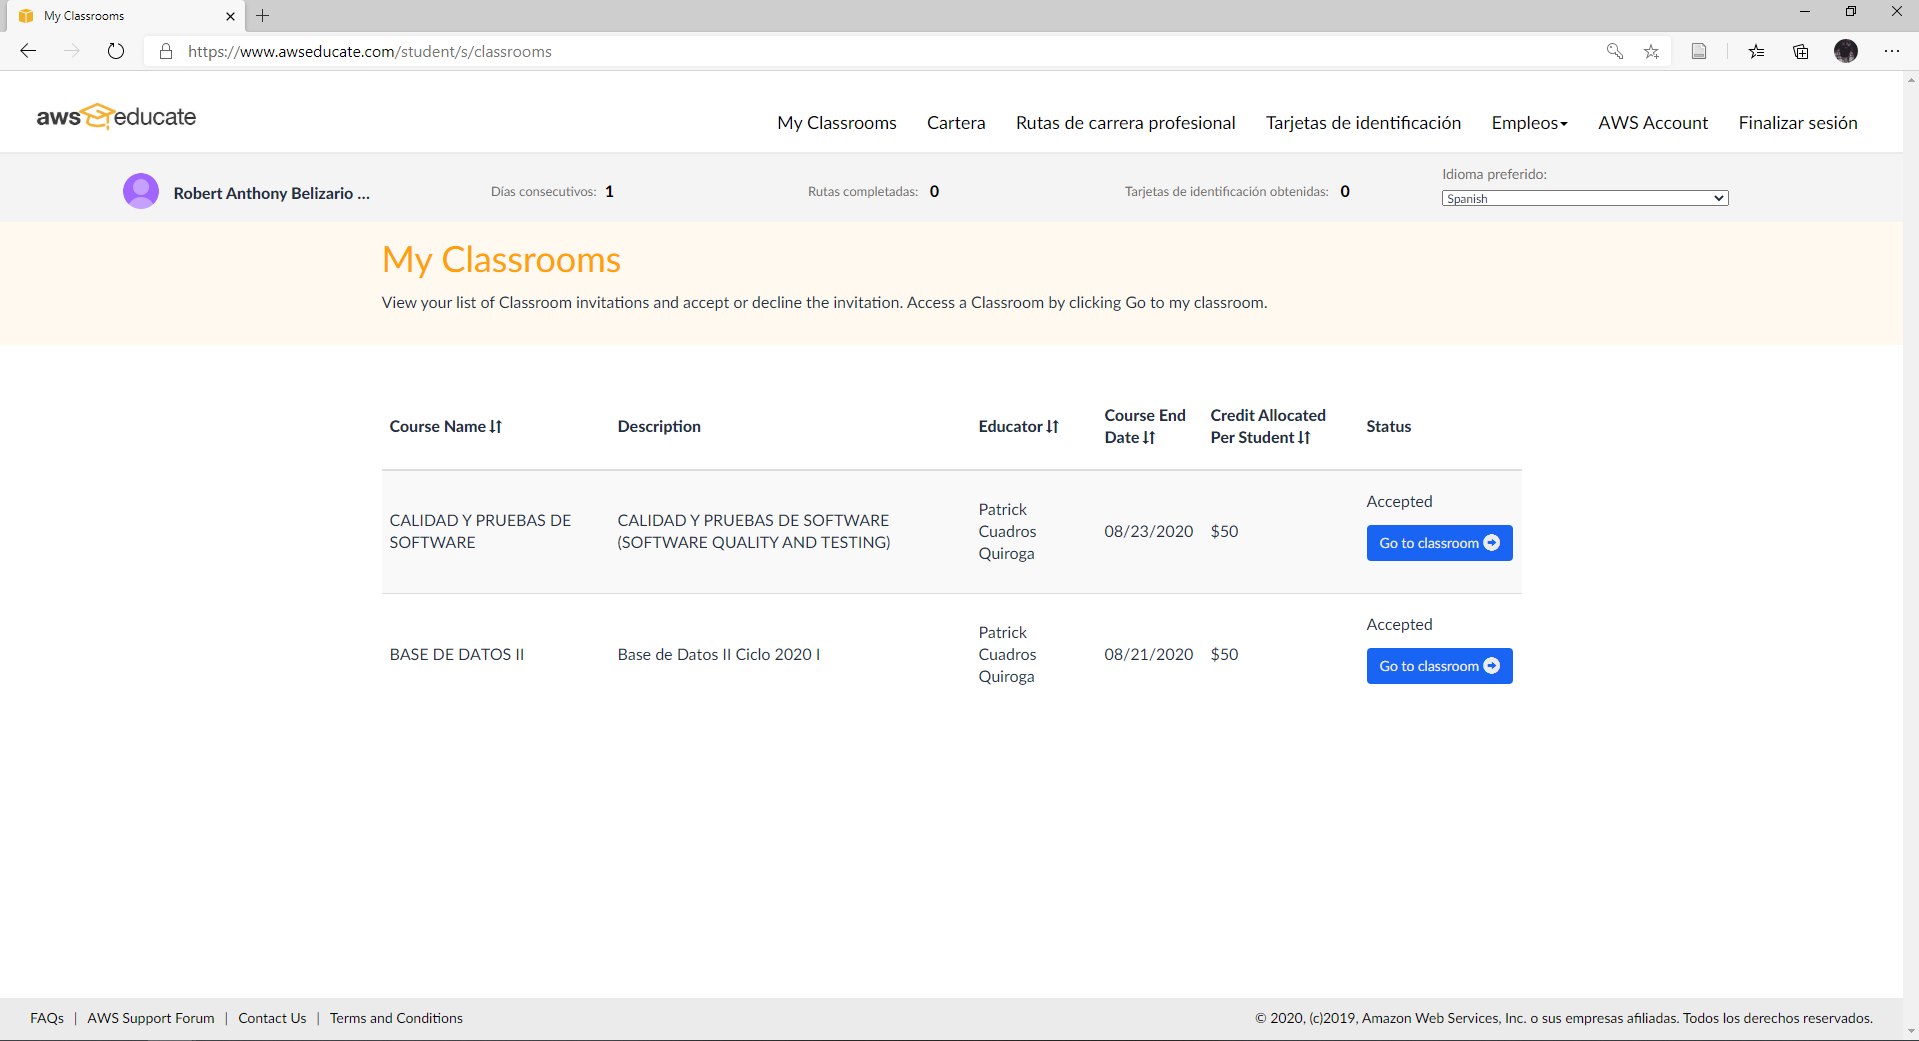
\includegraphics[width=15cm]{img/1.png}  
\end{center}




2.	Luego nos aparecera el estado de la clase, para hacer el laboratorio elegimos AWS Console.

\begin{center}
    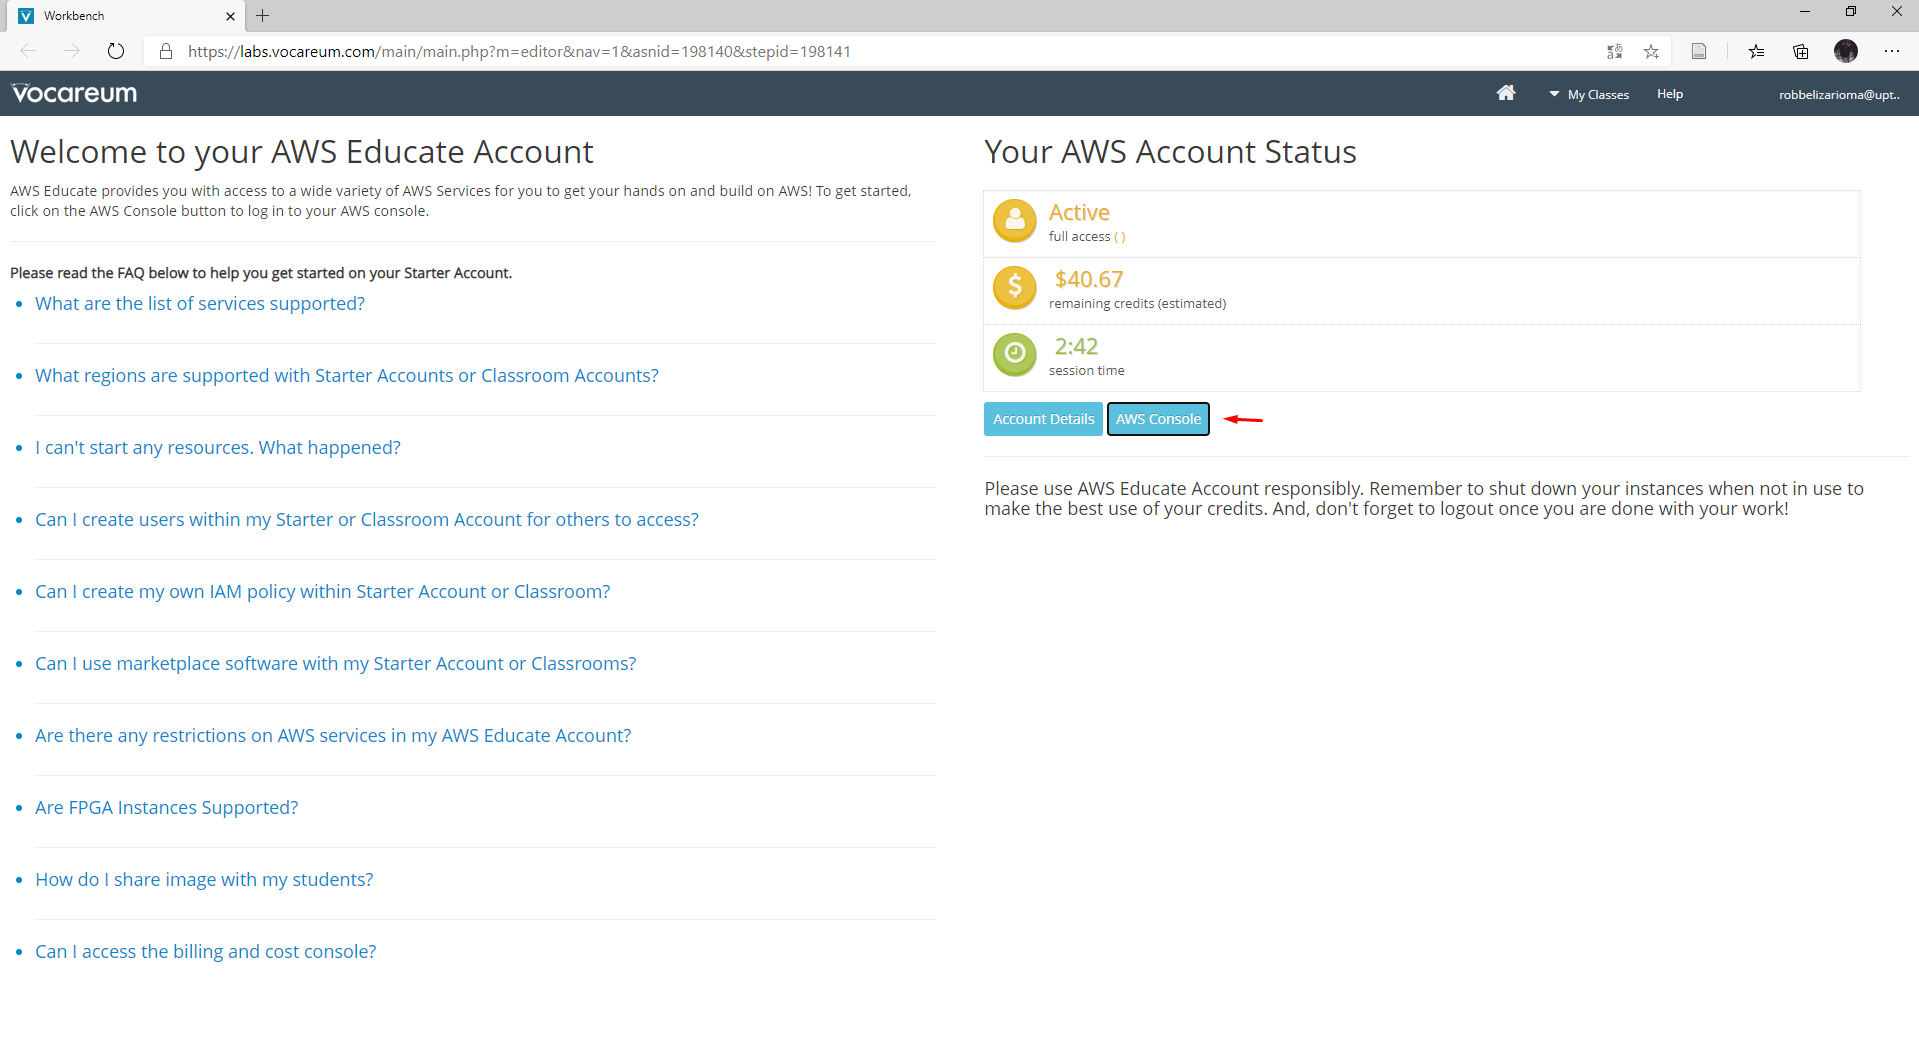
\includegraphics[width=15cm]{img/2.png}  
\end{center}
\newpage




3.	Primero en la consola de administración de AWS, buscamos DynamoDB.
\begin{center}
    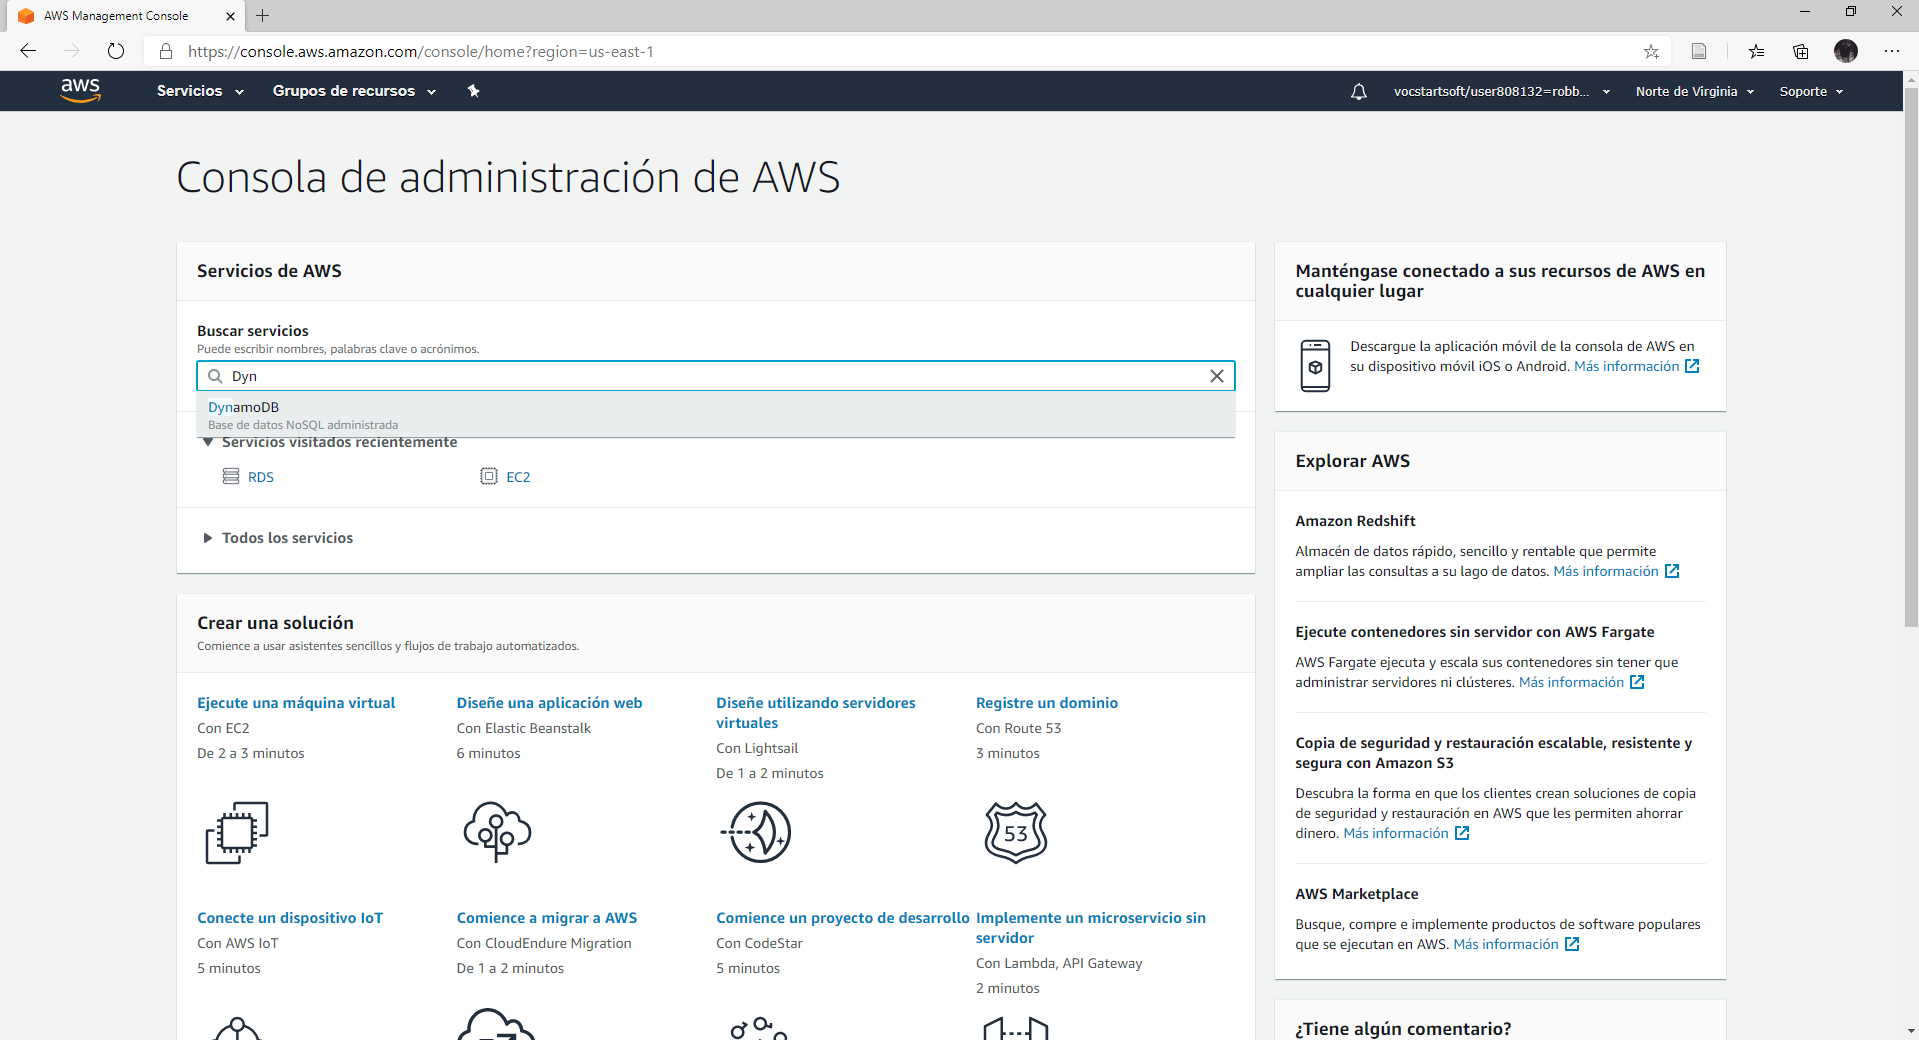
\includegraphics[width=15cm]{img/3.png}  
\end{center}




\section{ CREACION DE TABLA} 
4.	Ahora en la consola de DynamoDB, vamos a hacer click en crear tabla.
\begin{center}
    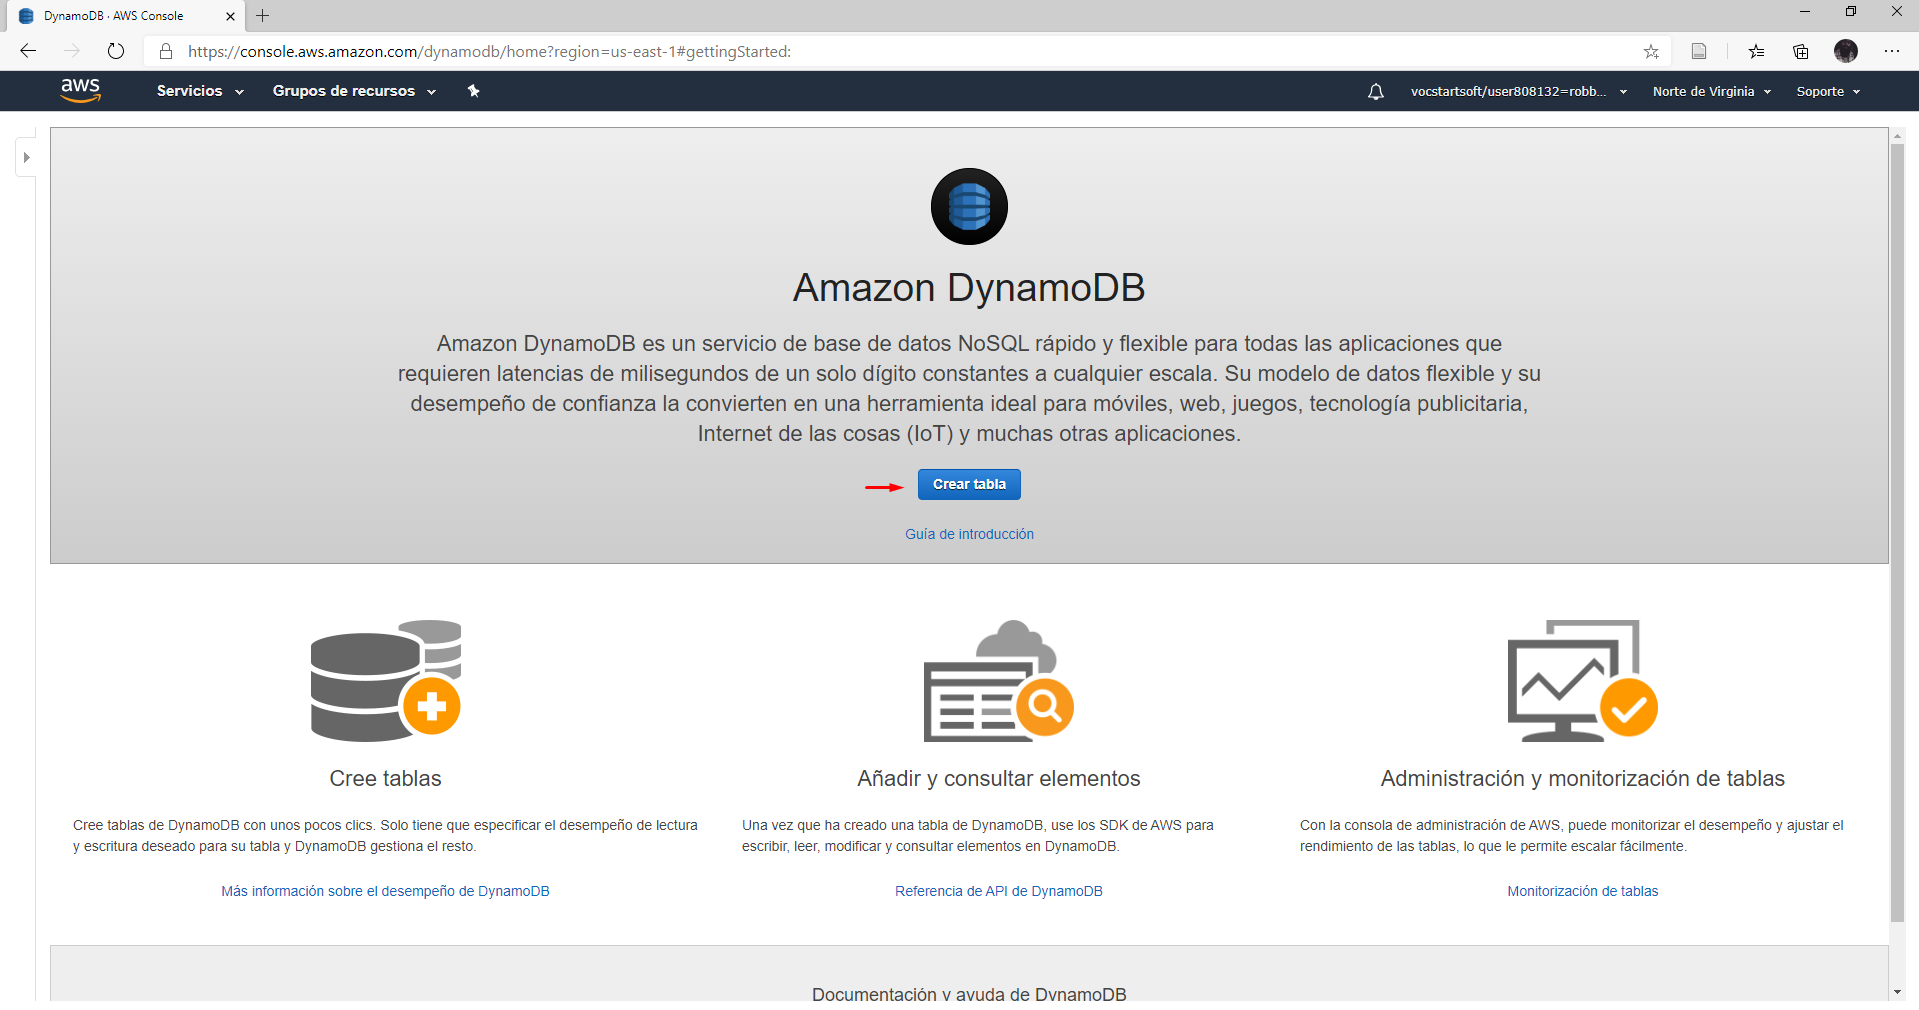
\includegraphics[width=15cm]{img/4.png}  
\end{center}
\newpage


5.	Como prueba vamos a utilizar una biblioteca de musica como nuestro caso de uso, el nombre de la tabla sera Music.
\begin{center}
    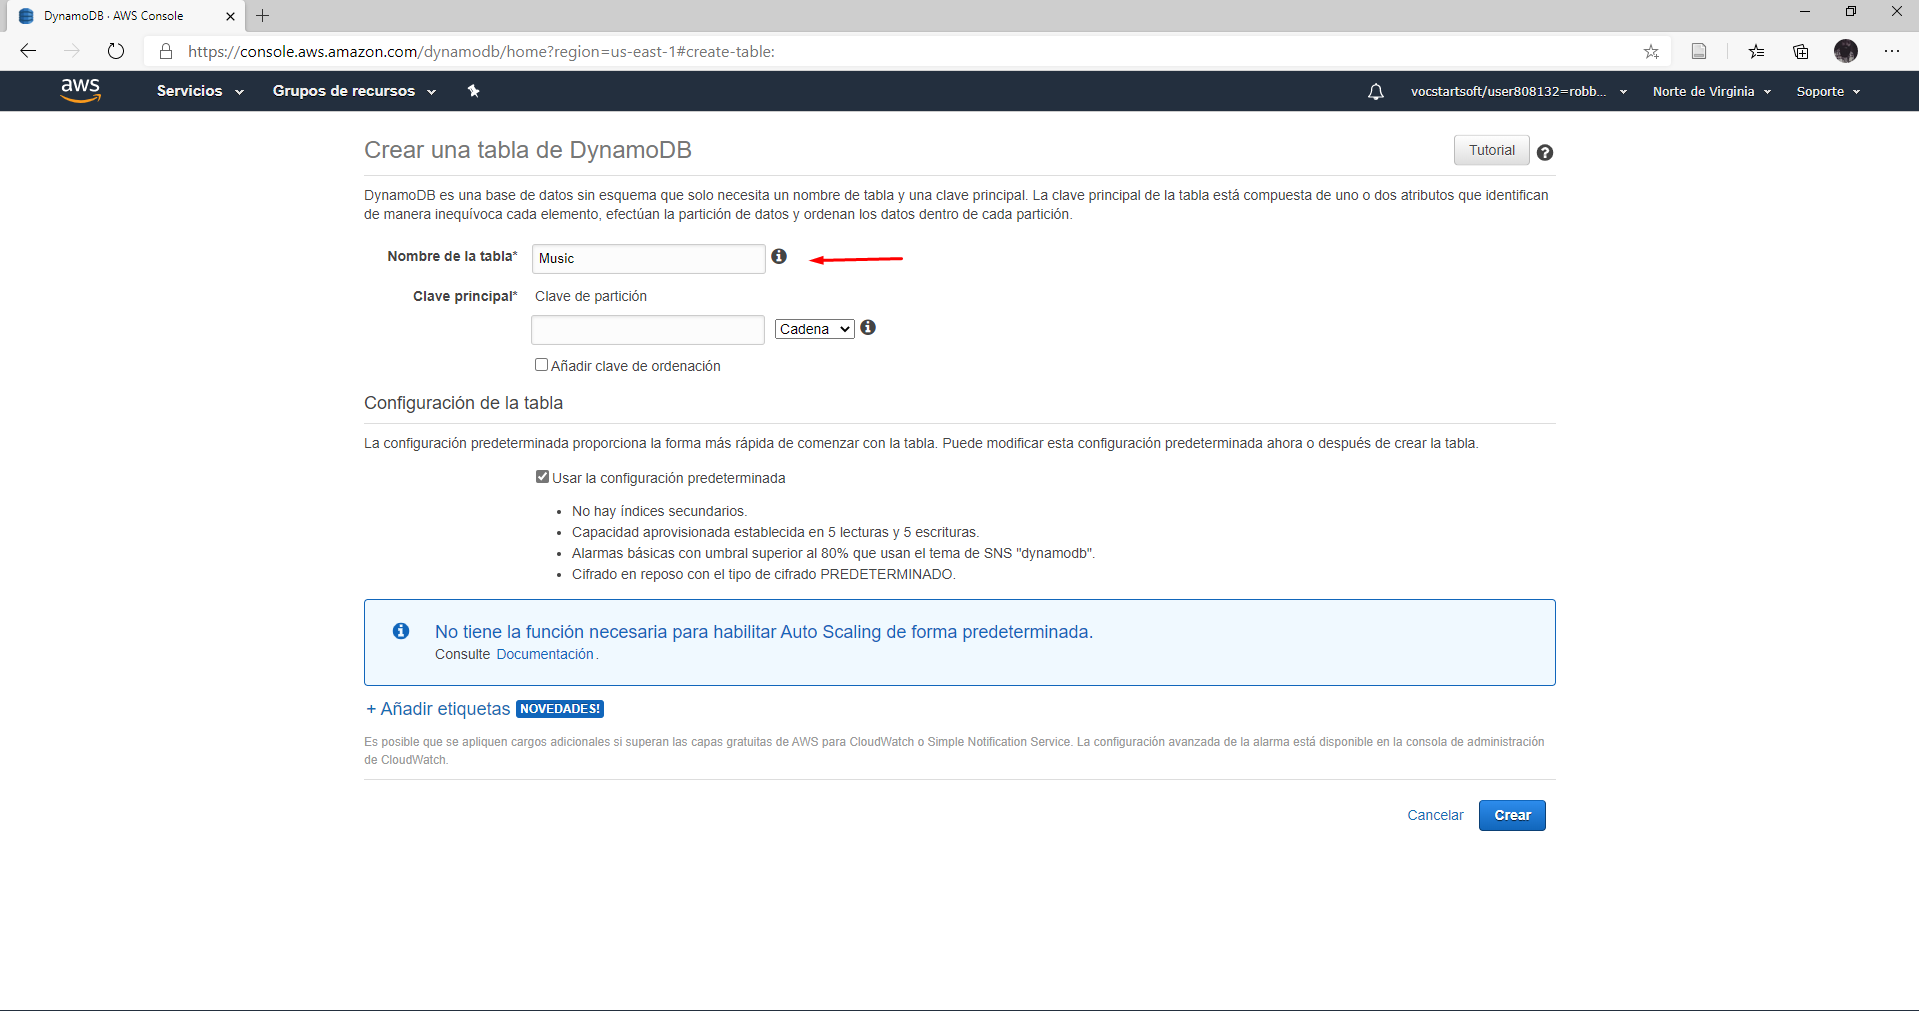
\includegraphics[width=15cm]{img/5.png}  
\end{center}





6.	En la clave de particion vamos a elegir un atributo con una amplia gama de valores, sera en este caso Artist tipo cadena o String.
\begin{center}
    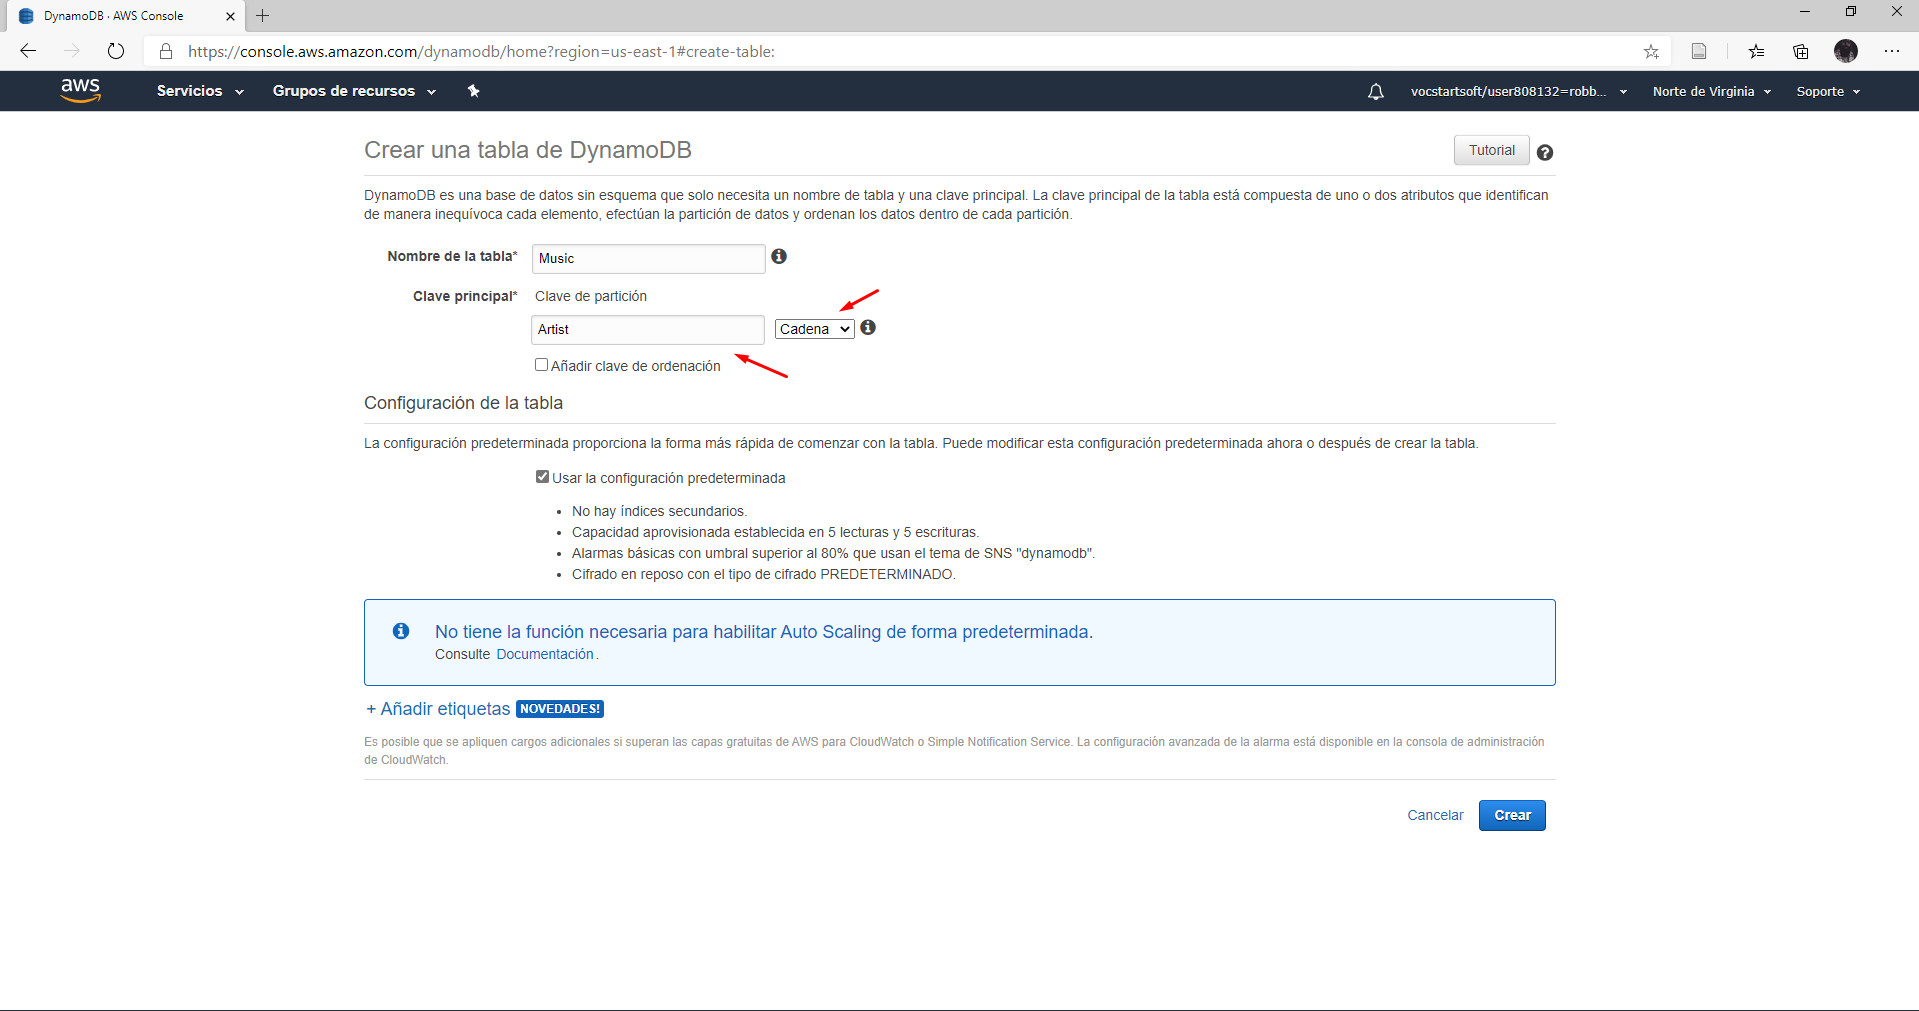
\includegraphics[width=15cm]{img/6.png}  
\end{center}
\newpage




7.	Como cada artista puede componer muchas canciones, puede habilitar el ordenamiento sencillo con una clave de ordenamiento. Añadiremos una clave de ordenamiento que sera SongTitle.
\begin{center}
    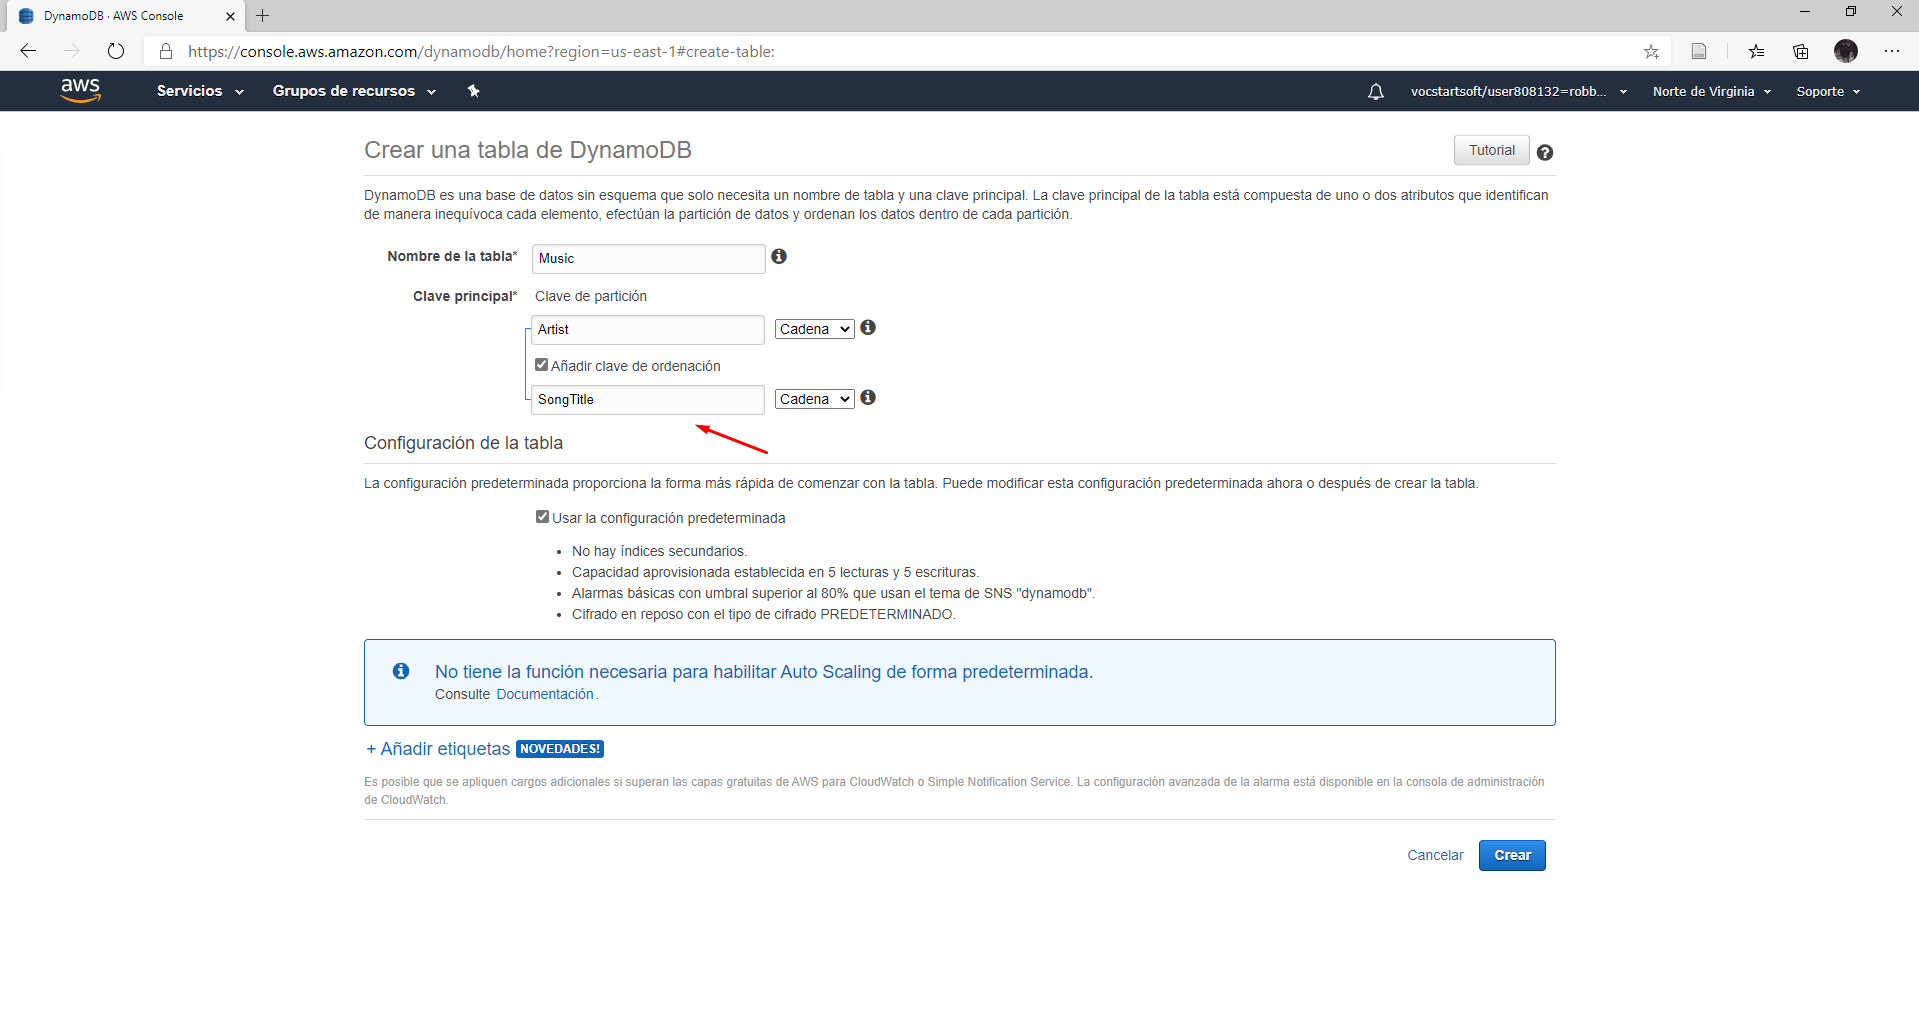
\includegraphics[width=15cm]{img/7.png}  
\end{center}




8.	Activaremos DynamoDB Auto Scaling para la tabla, esto modificara la capacidad de lectura y escritura de su tabla en funcion del volumen de solicitudes. Desmarcamos la configuracion recomendada.
\begin{center}
    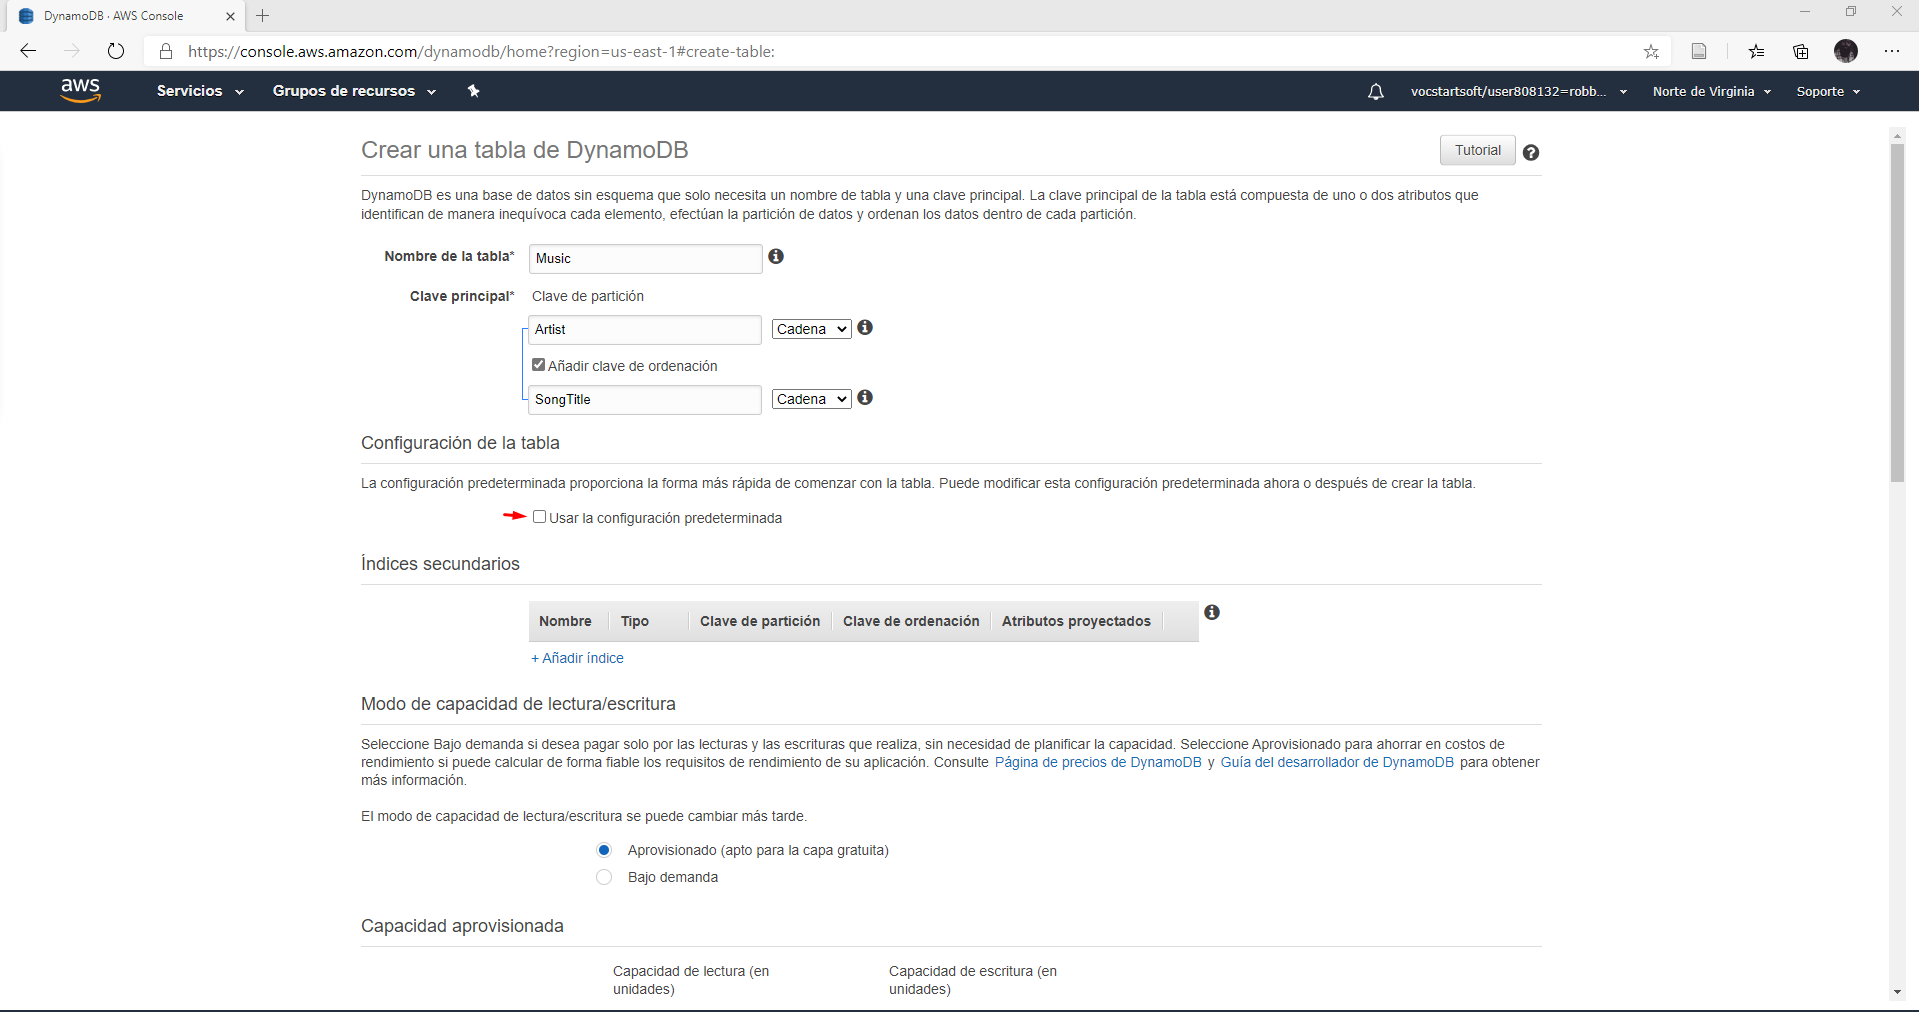
\includegraphics[width=15cm]{img/8.png}  
\end{center}
\newpage

9.	No modificaremos nada para los fines del tutorial.
\begin{center}
    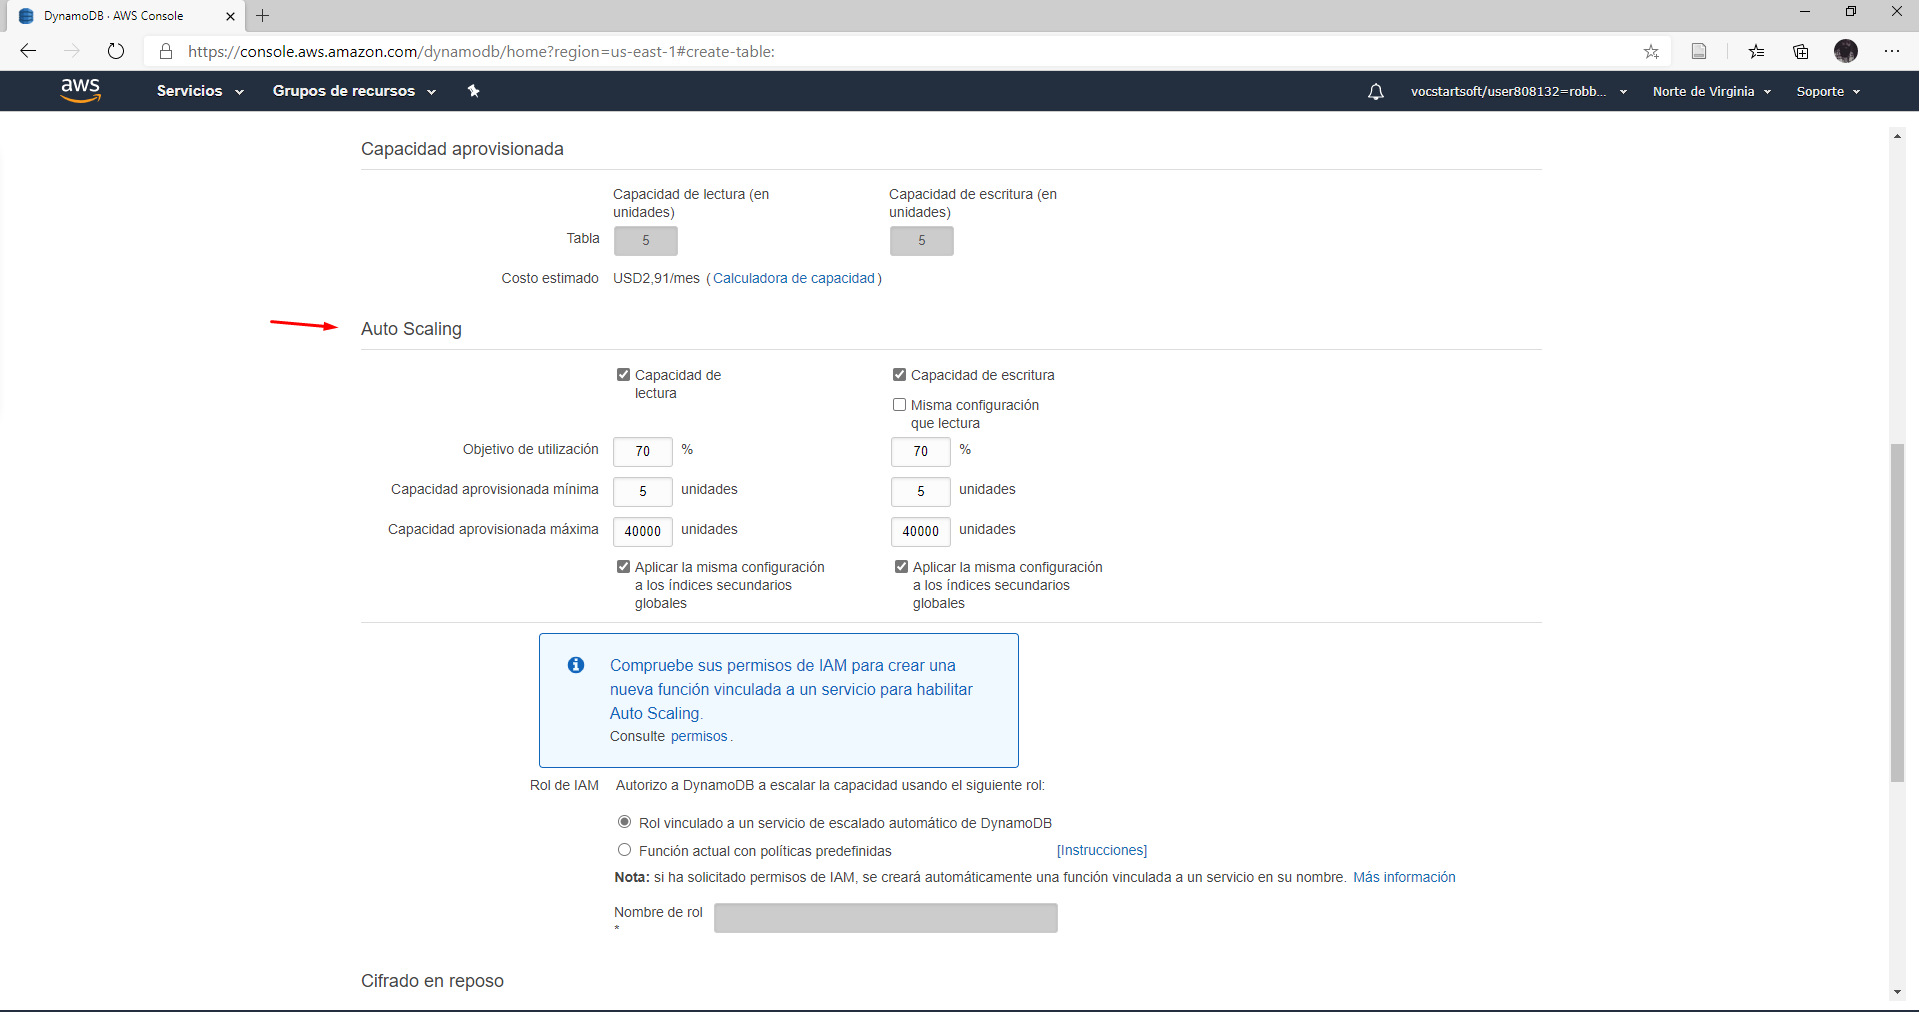
\includegraphics[width=15cm]{img/9.png}  
\end{center}


10.	Y ya le dariamos en CREAR.
\begin{center}
    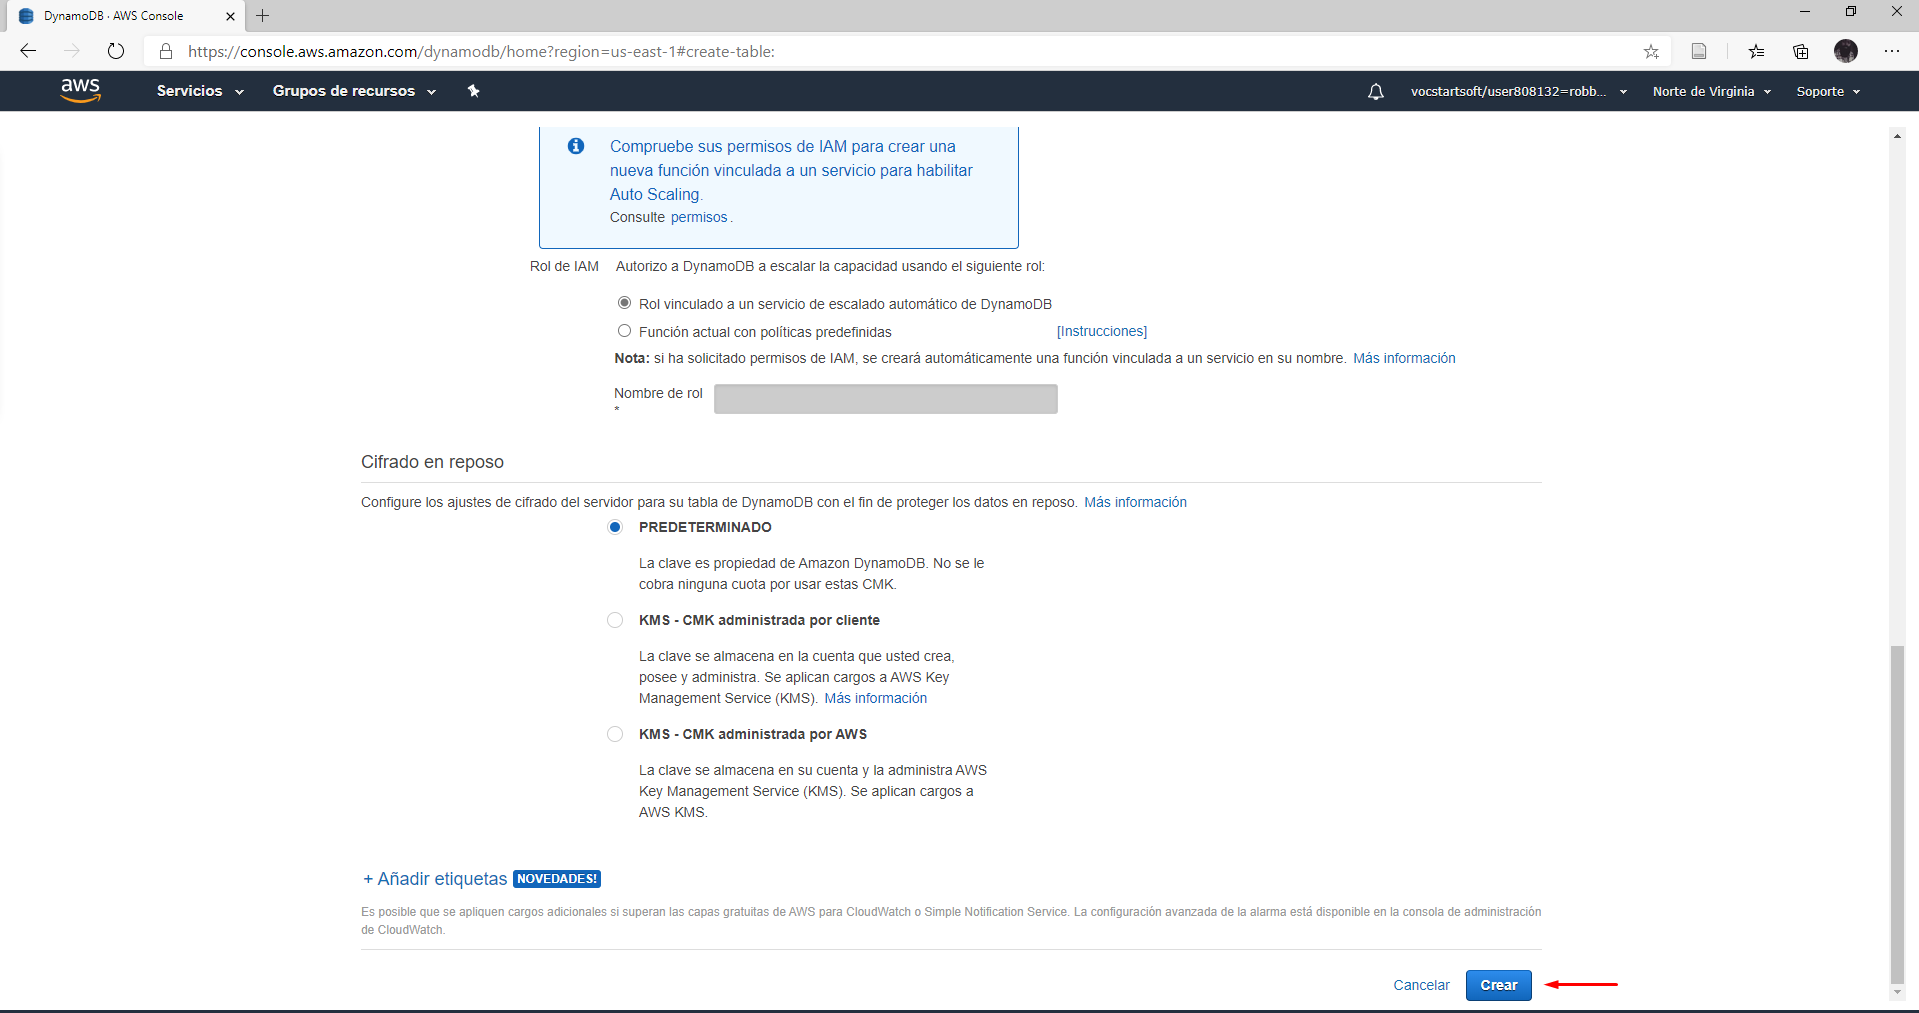
\includegraphics[width=15cm]{img/10.png}  
\end{center}
\newpage

\section{AGREGANDO DATOS A LA TABLA}
11.	Ahora vamos agregar datos a la tabla NoSQL
\begin{center}
    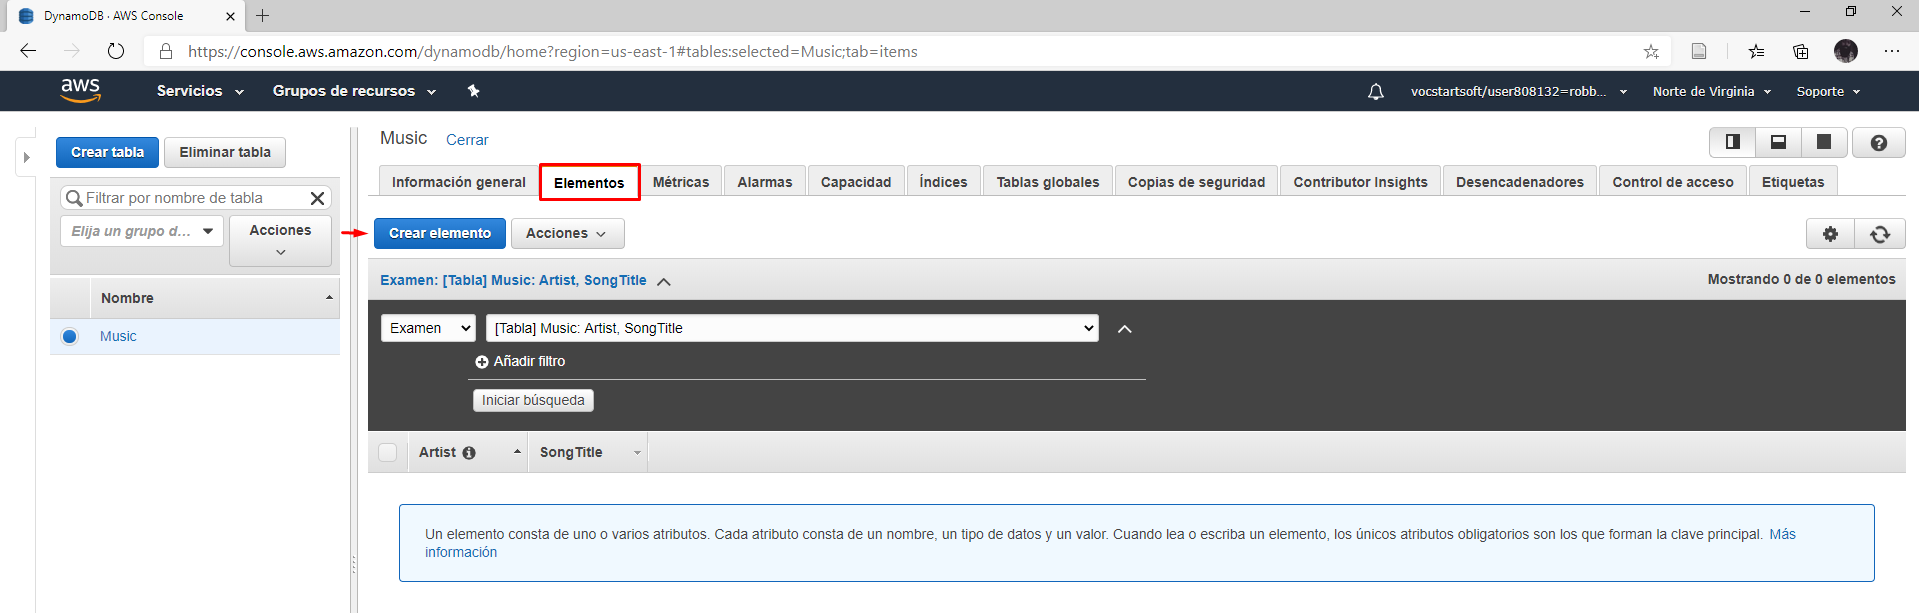
\includegraphics[width=15cm]{img/11.png}  
\end{center}


12.	En Artist ponemos No One You Know, y en SongTitle Call Me Today, como ejemplo y le damos a Guardar.
\begin{center}
    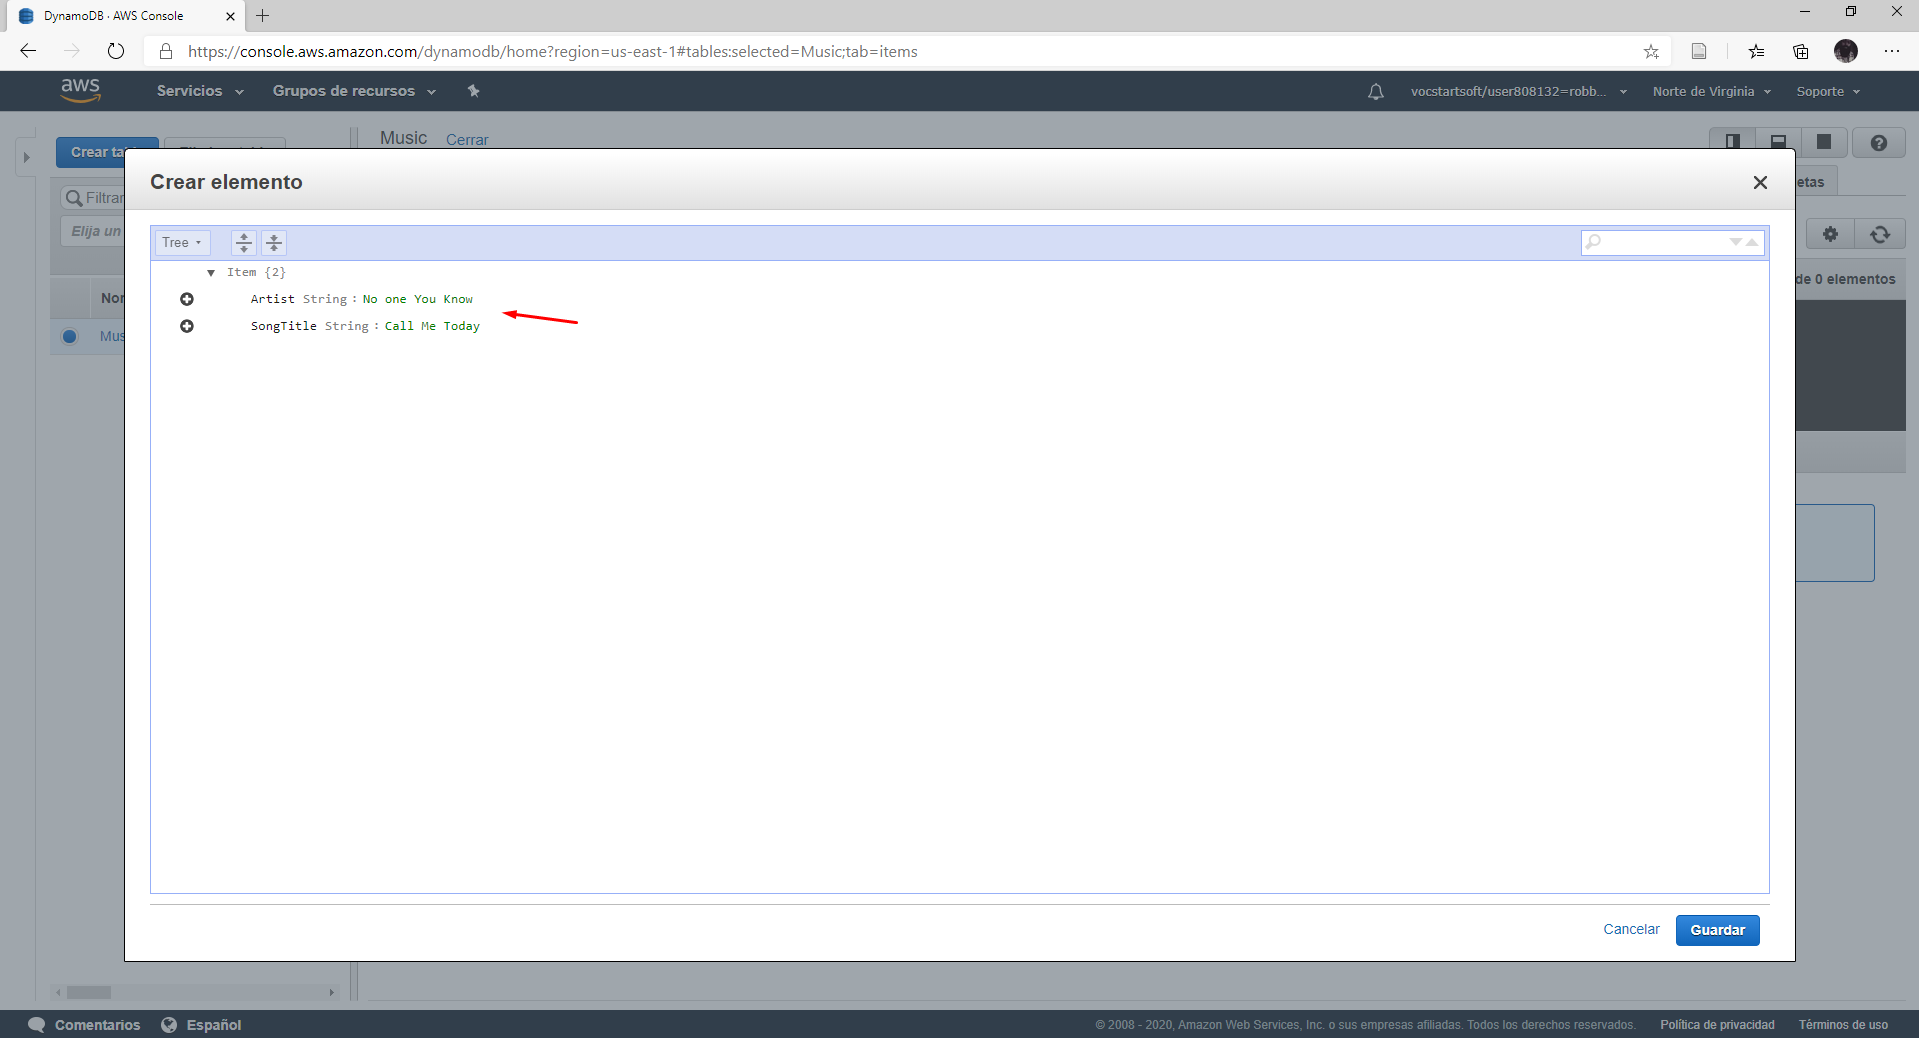
\includegraphics[width=15cm]{img/12.png}  
\end{center}


13.	Aqui lo veríamos creado
\begin{center}
    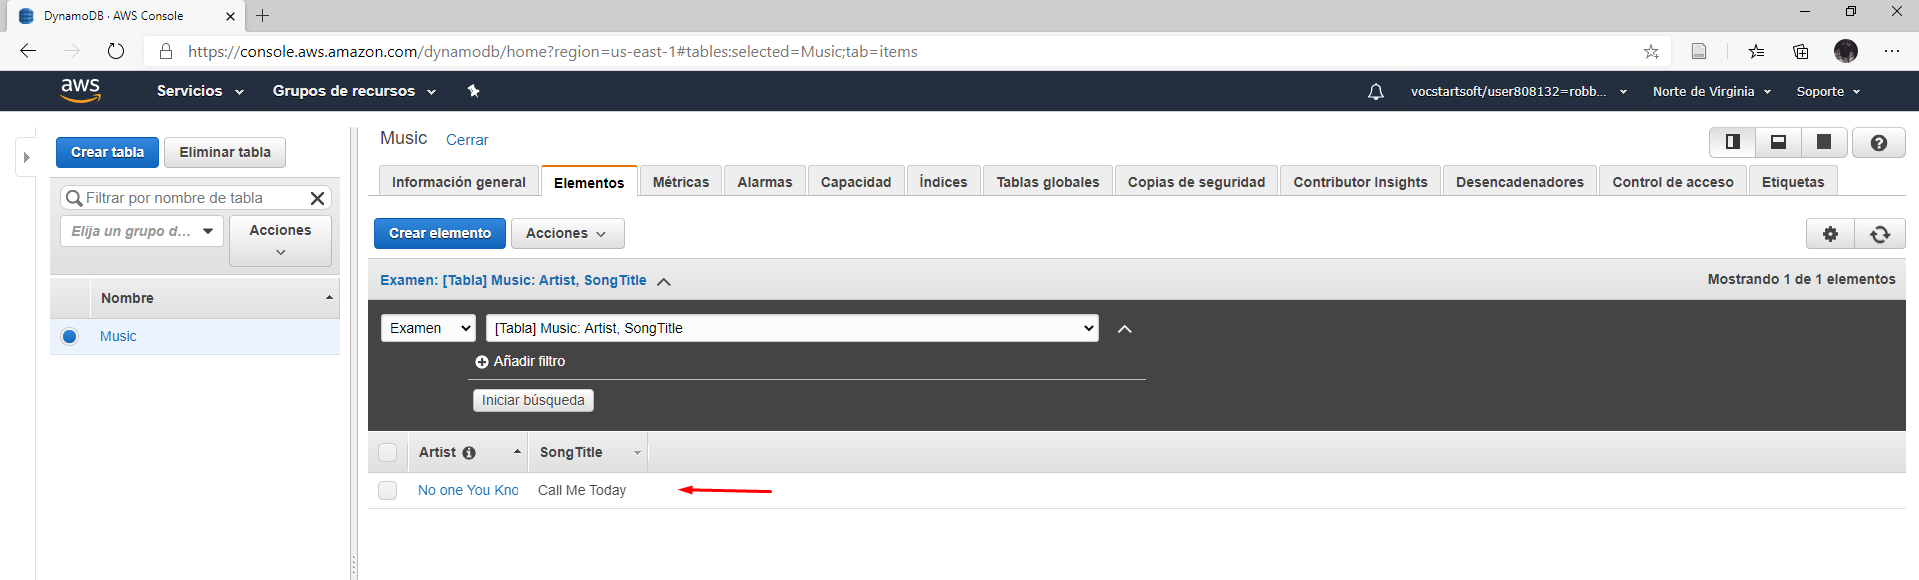
\includegraphics[width=15cm]{img/13.png}  
\end{center}
\newpage


14.	Agregaremos mas datos a la tabla Music.
\begin{center}
    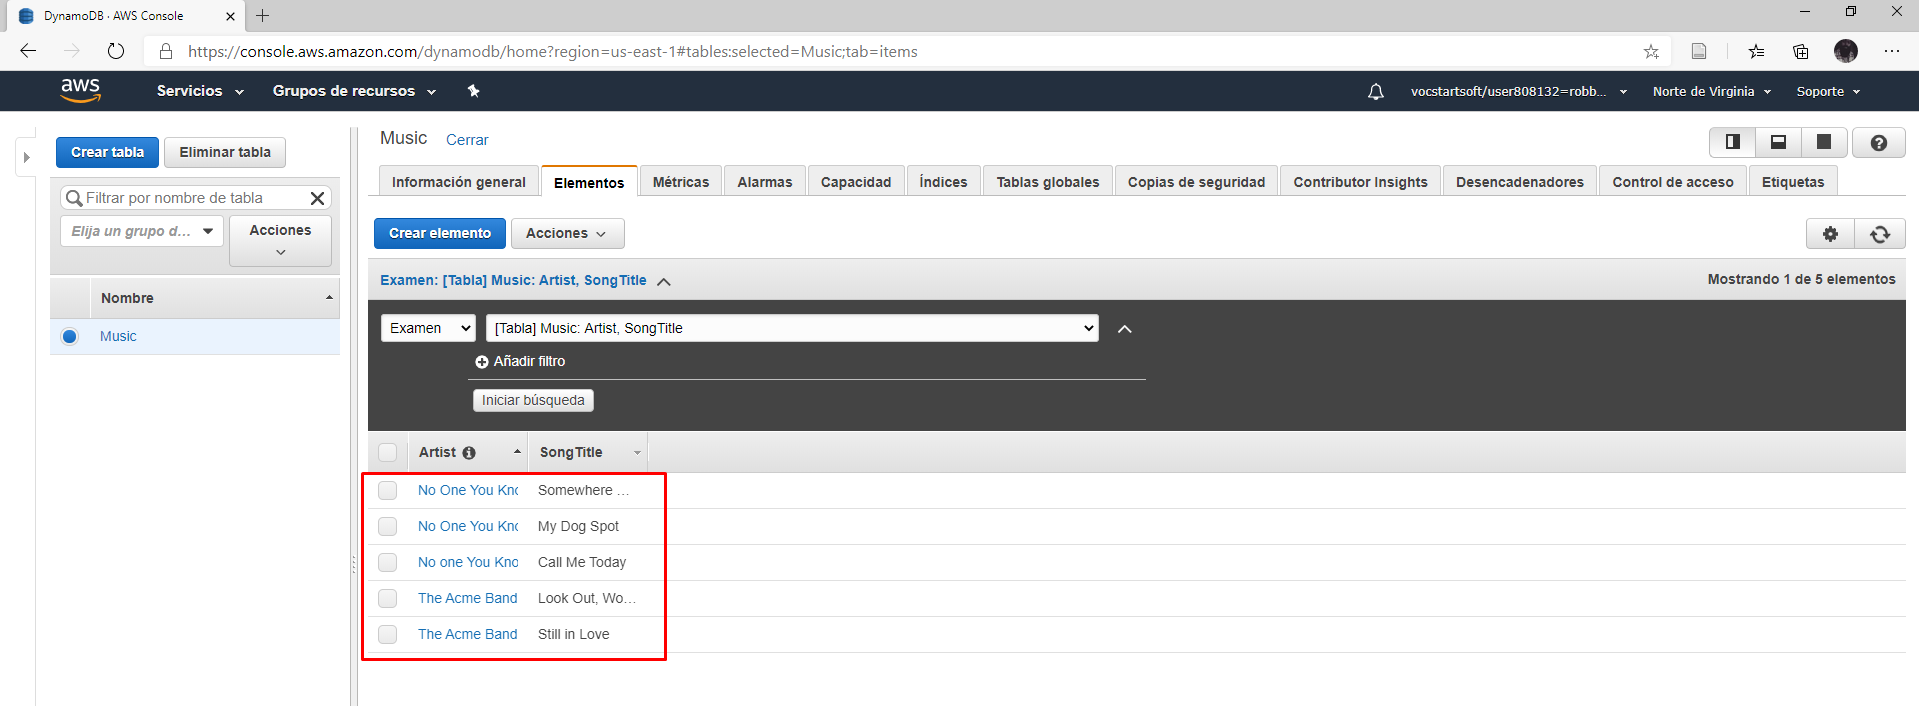
\includegraphics[width=15cm]{img/14.png}  
\end{center}
\newpage

\section{REALIZANDO CONSULTAS A LA TABLA}
15.	 Ahora pasaremos a realizar una consulta en la tabla NoSQL, seleccionamos consulta y mostraria lo siguiente.
\begin{center}
    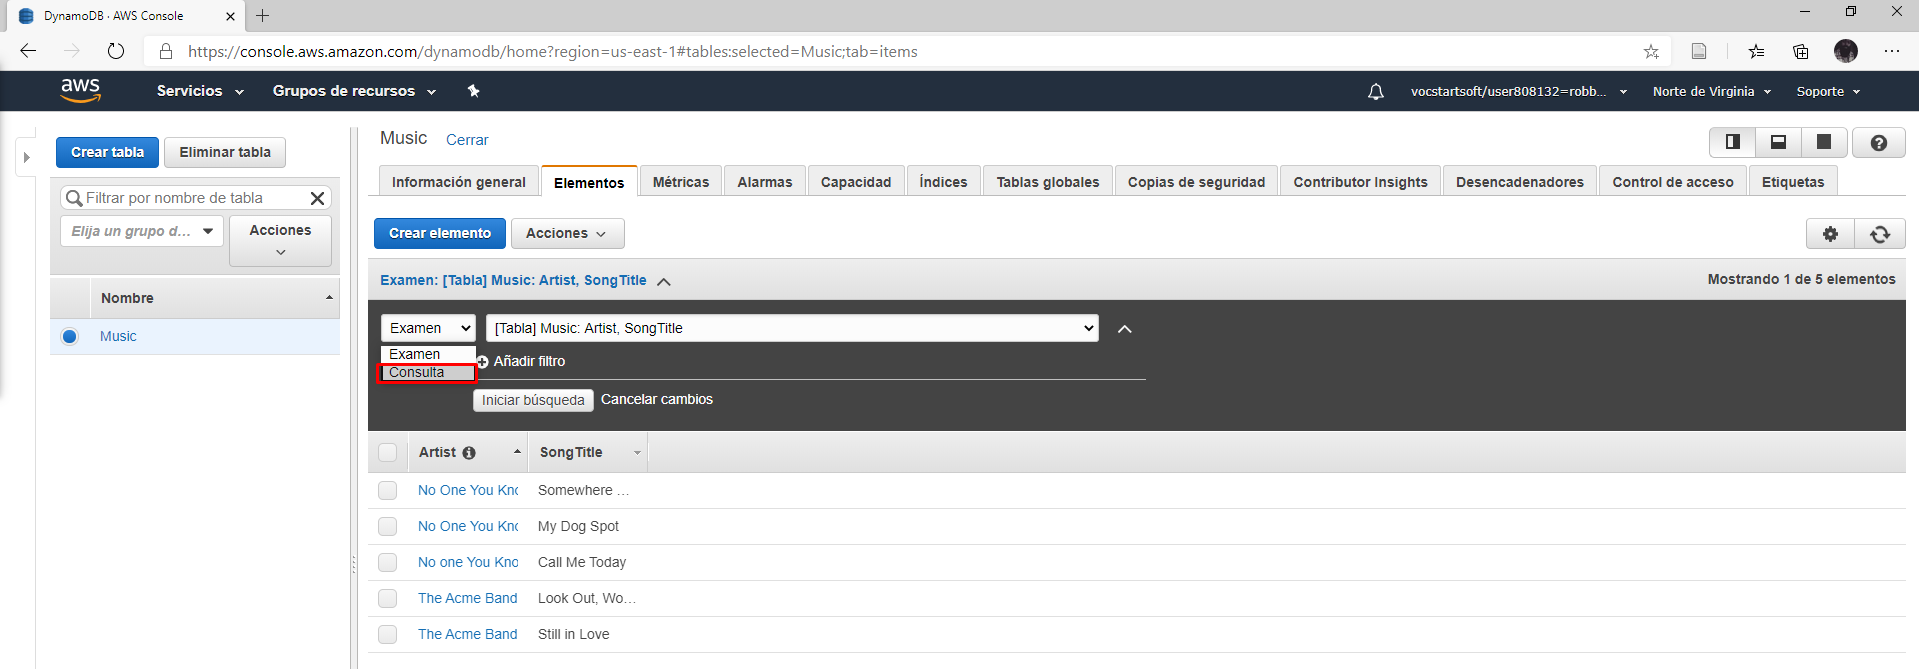
\includegraphics[width=15cm]{img/15.png}  
\end{center}
\begin{center}
    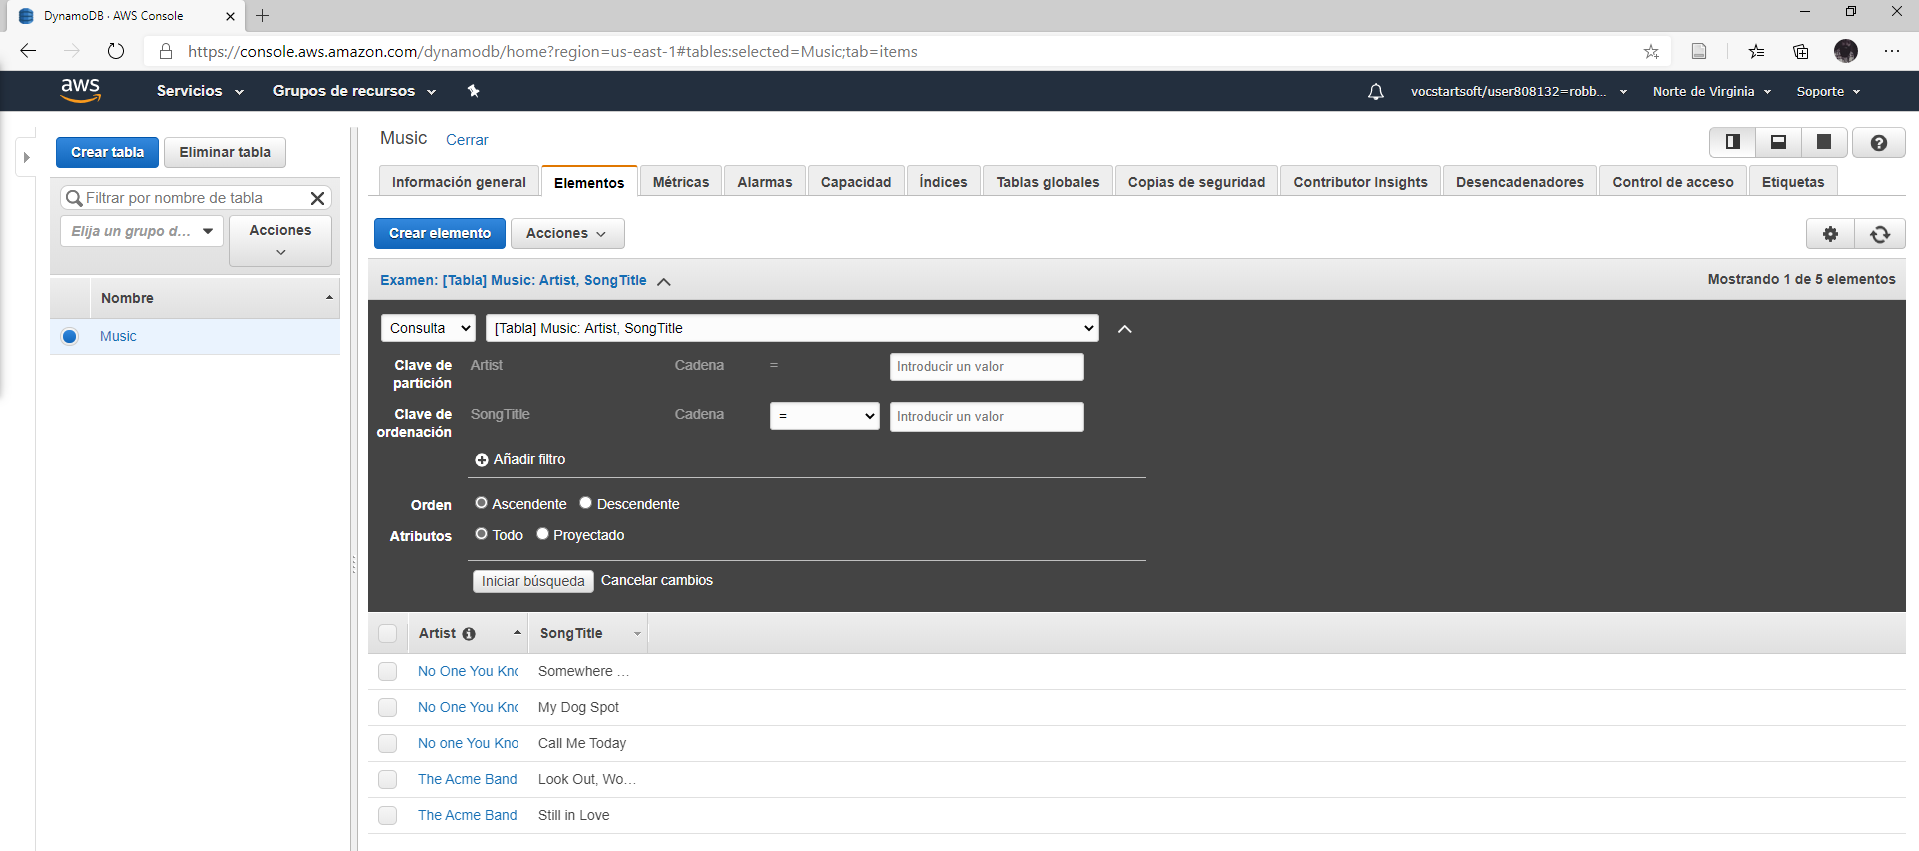
\includegraphics[width=15cm]{img/15.1.png}  
\end{center}


16.	Para la primera consulta en Artist escribiremos No One You Know, y procederemos a hacer click en Iniciar busqueda.
\begin{center}
    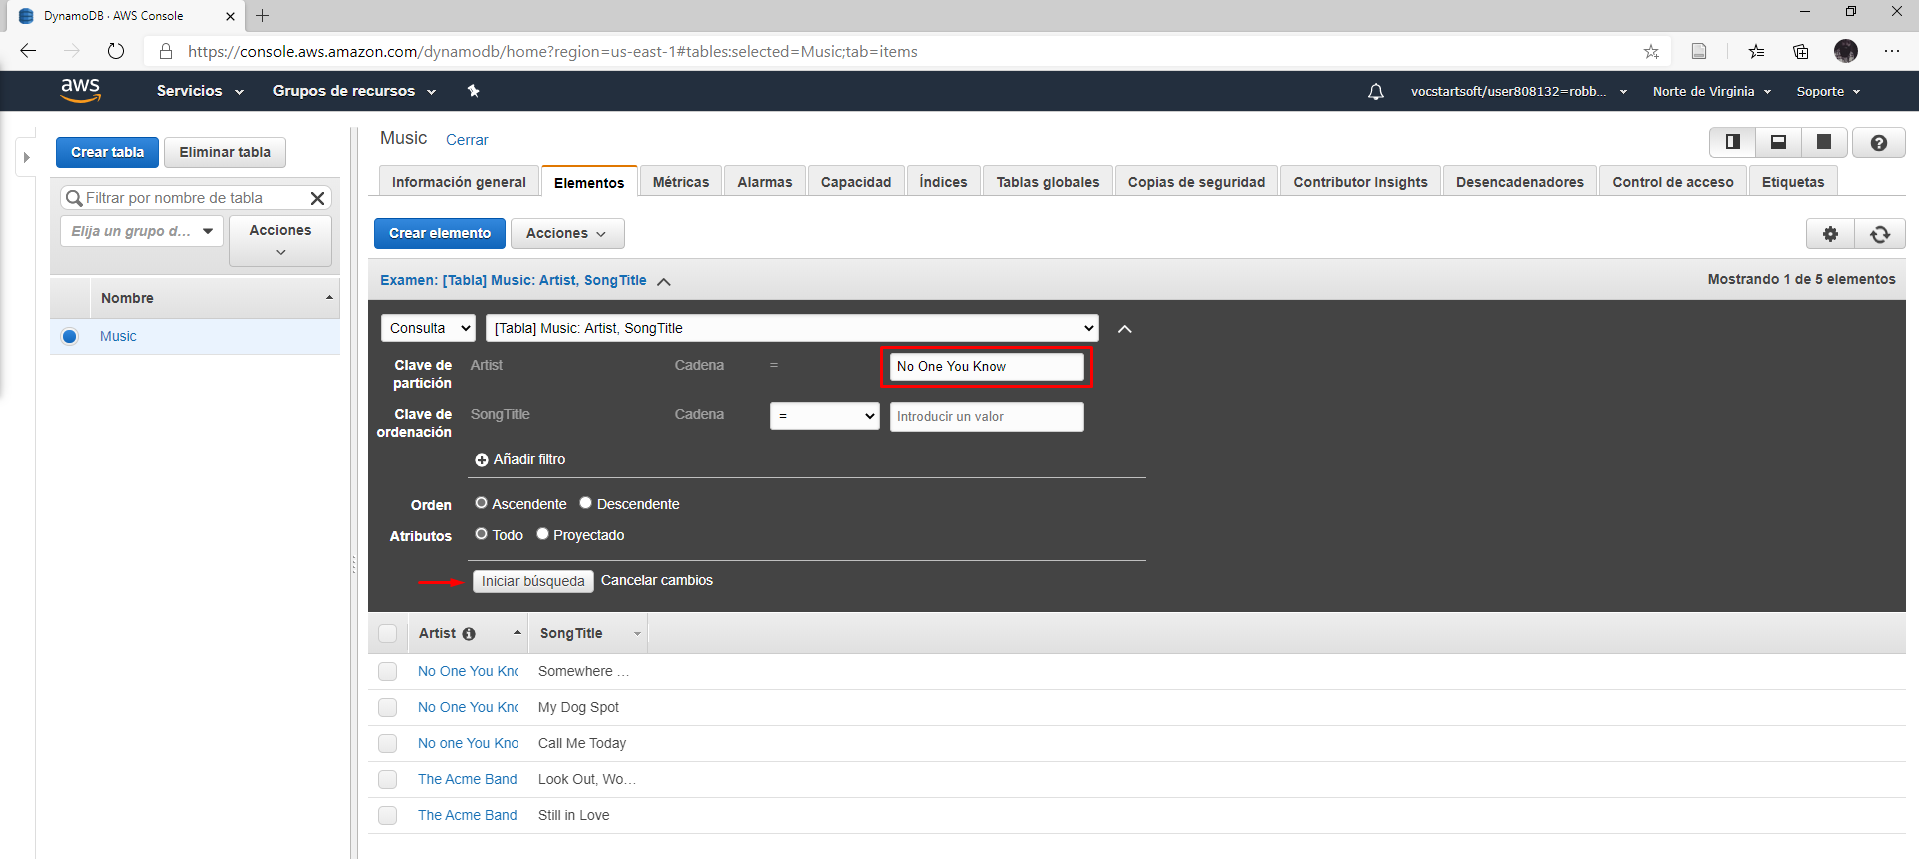
\includegraphics[width=15cm]{img/16.png}  
\end{center}
\newpage

17.	Vemos abajo los resultados de la busqueda.
\begin{center}
    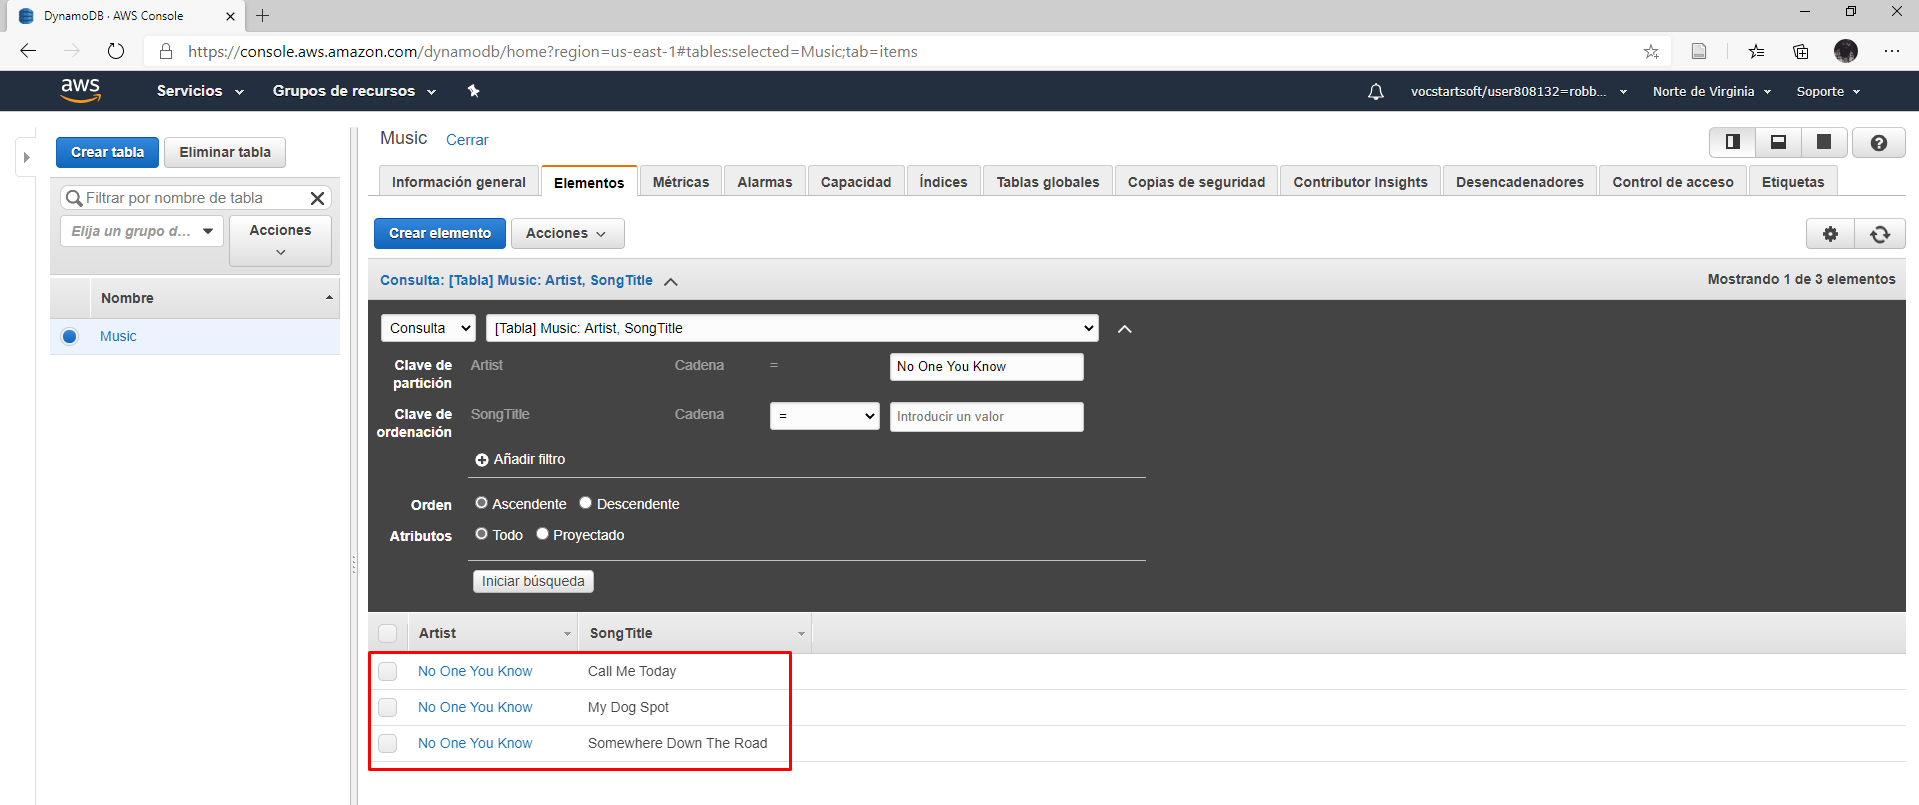
\includegraphics[width=15cm]{img/17.png}  
\end{center}


18.	Probaremos con otra, en Artist pondremos The Acme Band.
\begin{center}
    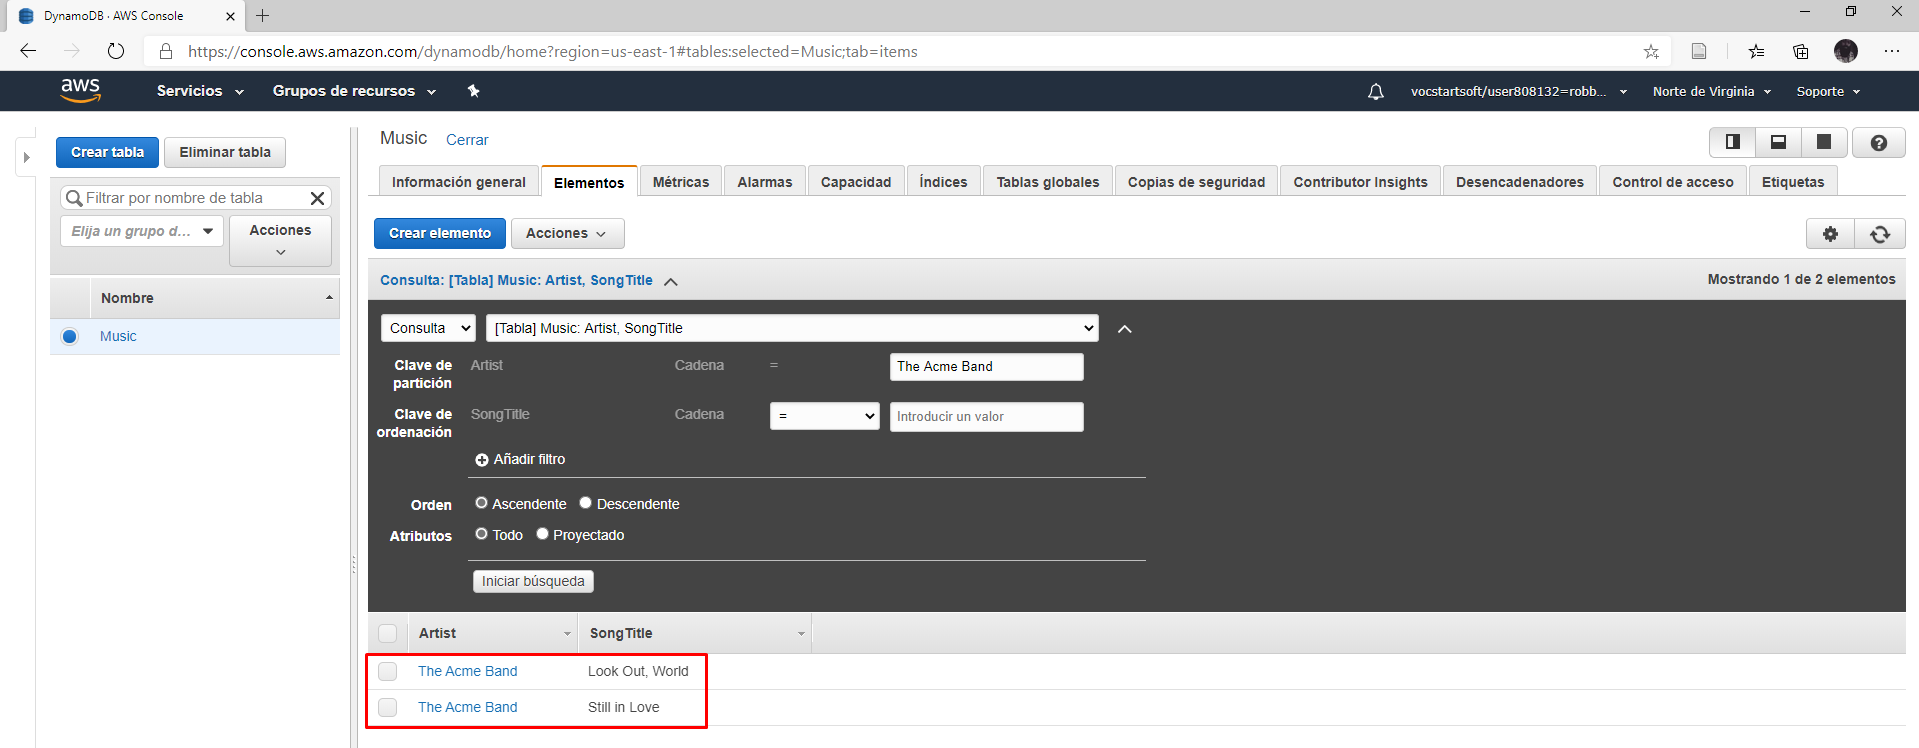
\includegraphics[width=15cm]{img/18.png}  
\end{center}
\newpage

\section{ELIMINANDO DATOS DE LA TABLA}
19.	Ahora probaremos eliminando un elemento, seleccionamos primero el elemento, luego en acciones elegimos Eliminar.
\begin{center}
    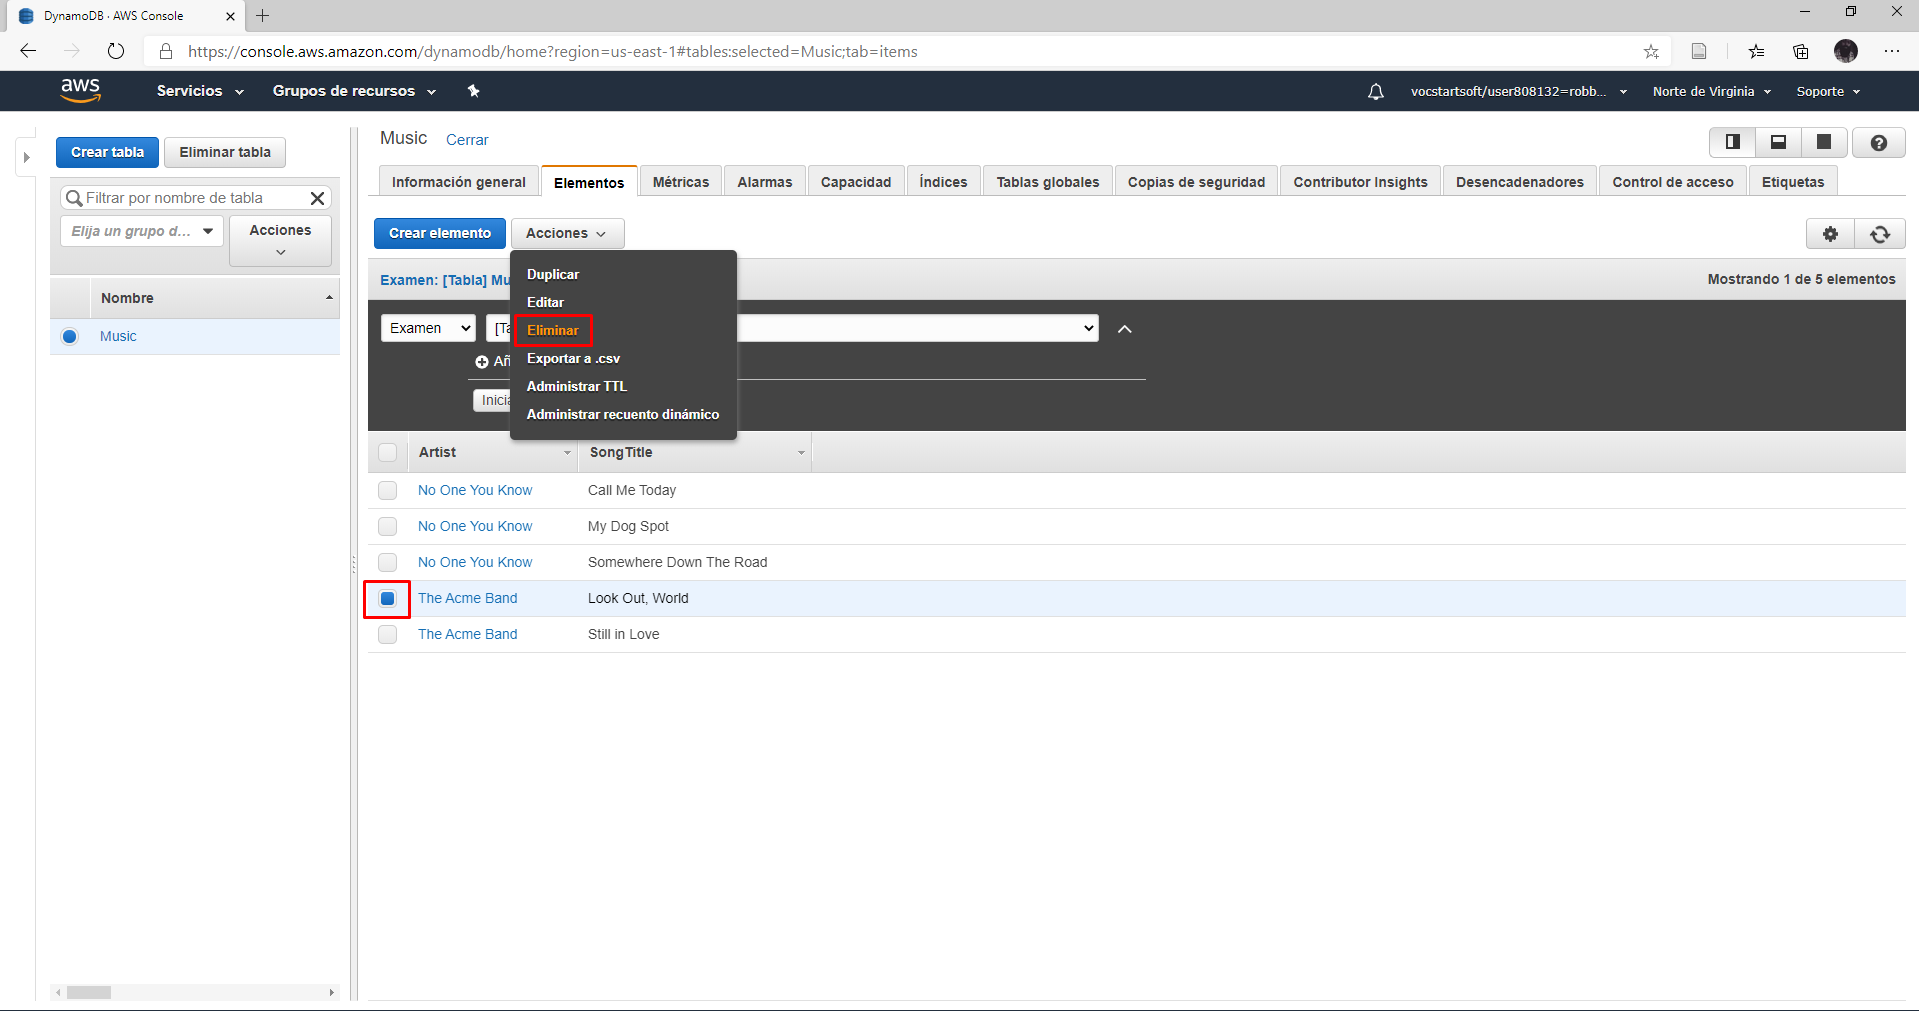
\includegraphics[width=15cm]{img/19.png}  
\end{center}
\begin{center}
    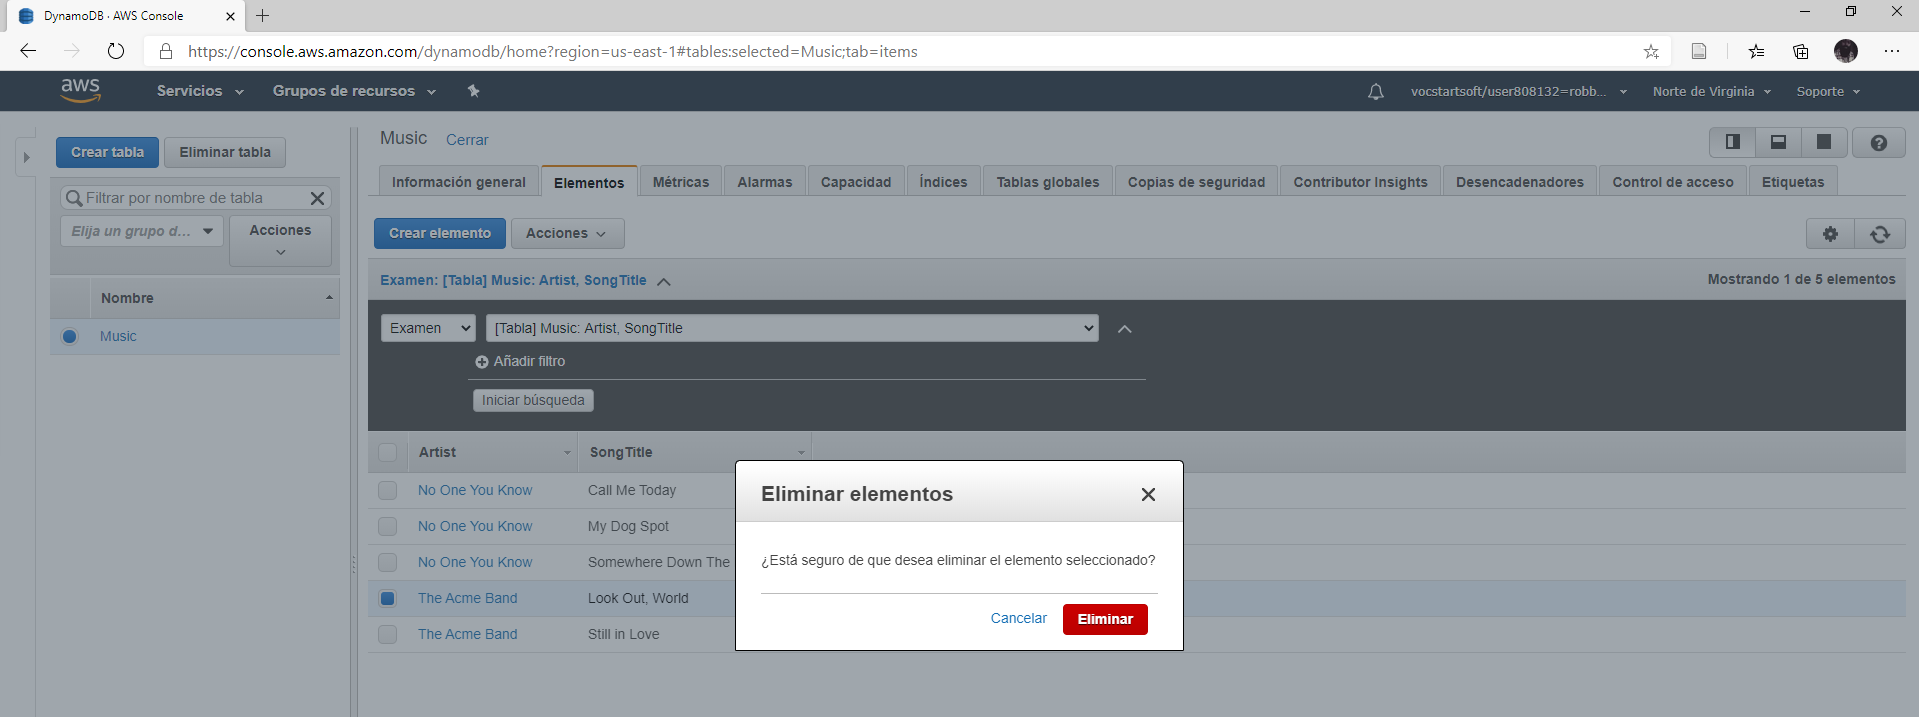
\includegraphics[width=15cm]{img/19.1.png}  
\end{center}
\newpage

\section{ELIMINANDO LA TABLA}
20.	Por ultimo pasaremos a eliminar una tabla, seleccionamos primero la tabla, apretamos en Eliminar tabla, escribimos delete para poder borrar y damos en eliminar.
\begin{center}
    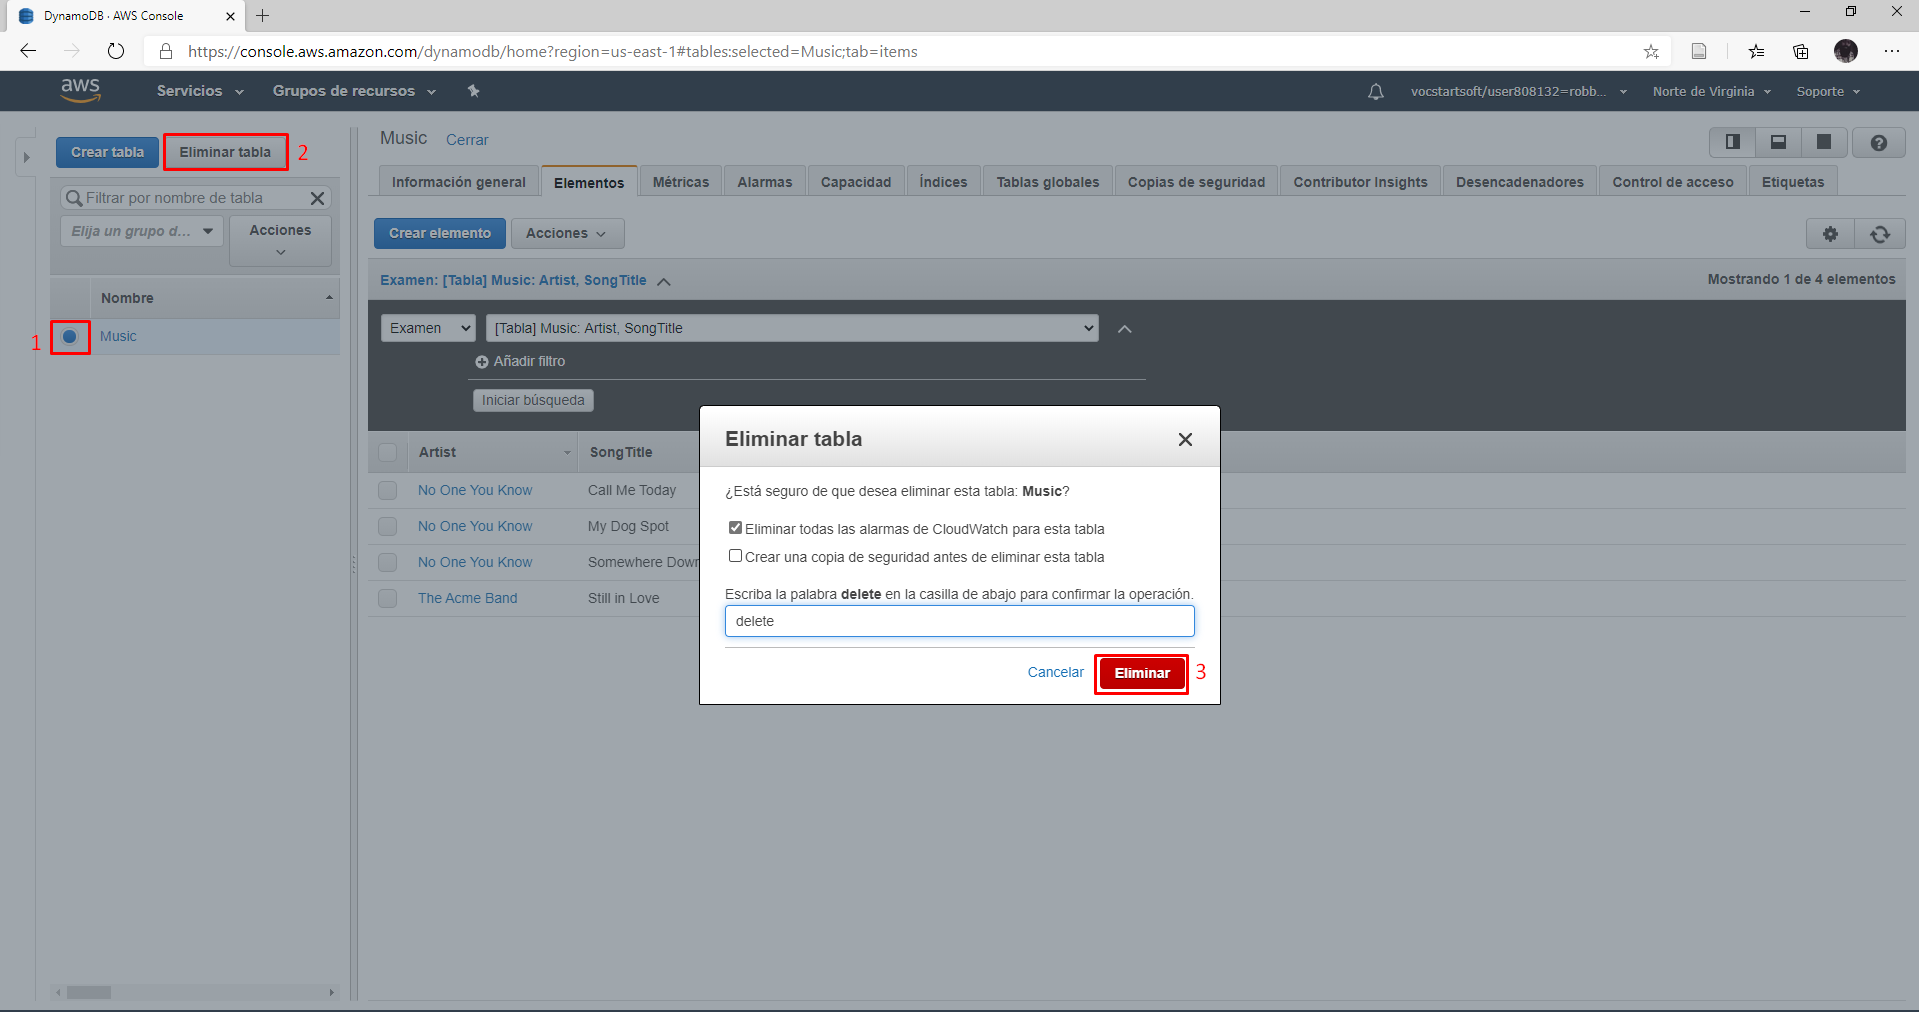
\includegraphics[width=15cm]{img/20.png}  
\end{center}
\end{document}

